\documentclass[11pt,twoside,fleqn,openright,titlepage]{cslreport}
%\topmargin 12pt
\topmargin .2in
\textwidth 5.5in
\textheight 7.75in
\oddsidemargin .65in
\evensidemargin .41in
\marginparwidth 0.85in
\marginparsep 0.2in

\raggedbottom
\usepackage{cite,relative,alltt,times}
\usepackage{amsfonts,latexsym,amssymb}
\usepackage{xcolor}
\definecolor{lgrey}{gray}{0.98}

\usepackage{listings}
\lstset{basicstyle=\ttfamily,showstringspaces=false,frame=single,backgroundcolor=\color{lgrey}}


\pagenumbering{roman}
\setcounter{page}{0}
\usepackage[bookmarks=true,hyperindex=true,colorlinks=true,linkcolor=black,citecolor=blue,urlcolor=blue]{hyperref}

%% \renewcommand{\baselinestretch}{1.5}

%%
%% Environment to list command-line arguments of a tool
%% (this is based on the \newenvironment{description} from report.cls)
%%
\newenvironment{options}{
\begin{list}{}{
\setlength{\labelsep}{1.8ex}
\setlength{\labelwidth}{0pt}
\setlength{\itemindent}{-0.5\leftmargin}
\settowidth{\leftmargin}{\texttt{--}}
\renewcommand{\makelabel}{\optionlabel}}}
{\end{list}}
\newcommand*\optionlabel[1]{\hspace\labelsep\texttt{#1}}

%%
%% hyphen in Math mode for things like (bool-to-bv ...)
%%
\mathchardef\mhyphen="2D

%%
%% Macros for naturals, integers, reals
%%
\newcommand{\integers}{\ensuremath{\mathbb{Z}}}
\newcommand{\naturals}{\ensuremath{\mathbb{N}}}
\newcommand{\reals}{\ensuremath{\mathbb{R}}}
\newcommand{\rationals}{\ensuremath{\mathbb{Q}}}


\begin{document}
\begin{titlepage}
\date{\today}
\author{Bruno Dutertre}
\title{\textbf{Yices Manual\\[0.6em]
Version 2.6.2}}
\end{titlepage}

\maketitle
\cleardoublepageblank
\tableofcontents
%\listoffigures
\cleardoublepage
\setcounter{page}{0}
\pagenumbering{arabic}


%%%%%%%%%%%%%%%%%%%%%%%%%%%%%%%
\chapter{Introduction}
%%%%%%%%%%%%%%%%%%%%%%%%%%%%%%%

This  manual   is  an  introduction   to  the  logic,   language,  and
architecture  of the  Yices~2 SMT  solver. Yices  is developed  at SRI
International's  Computer Science  Laboratory.   Since version  2.5.3,
Yices  is released  under the  GNU  General Public  License version  3
(reproduced  in   Appendix~\ref{license}).   Previous   versions  were
released   under  different   terms,  and   were  free-of-charge   for
non-commercial use.

\medskip\noindent
To discuss alternative license terms, please contact us at
\texttt{fm-license@csl.sri.com}.


\section{Download and Installation}

The latest stable version of Yices~2 can be downloaded at
\url{https://yices.csl.sri.com}.  We provide pre-compiled binaries for
the platforms and operating systems listed in Table~\ref{versions}. We
also provide source code there. For MacOS and Linux, you can also
install Yices~2 using package managers (i.e., homebrew for the Mac and
apt for Debian/Ubuntu).

\medskip\noindent
For the latest developments, you can clone our Git repository
\url{https://github.com/SRI-CSL/yices2}.


\subsection{Binary Distributions}

\begin{table}
\begin{center}
\renewcommand{\arraystretch}{1.1}
\begin{tabular}{|l|l|}
\hline
\textbf{OS/Hardware} & \textbf{Notes} \\
\hline
\hline
Linux 64 bits & Kernel 2.6.24 or more recent \\
\hline
Mac~OS~X 64 bits &  Mac~OS~X El Capitan\\
\hline
Windows (64 bits) & \\
\hline
\end{tabular}
\end{center}
\caption{Binary Distributions}
\label{versions}
\end{table}

To download stable Yices~2 binaries, go to
\url{https://yices.csl.sri.com} and select the distribution that you
want to install.  Untar or unzip the file and follow the instructions
in the included README file.  The binary distributions are
self-contained and do not require installation of third-party
libraries.

\medskip\noindent
To complete installation on Linux or Mac~OS~X, the binary
distributions include a shell script called \texttt{install-yices}. By
default, this script installs Yices in \texttt{/usr/local}. If
this is fine for you, type
\begin{small}
\begin{lstlisting}[language=sh]
   sudo ./install-yices
\end{lstlisting}
\end{small}
This will install the binaries in \texttt{/usr/local/bin}, the library
in \texttt{/usr/local/lib}, and the header files in
\texttt{/usr/local/include}.

\medskip\noindent
To install Yices in a different location, you can type
\begin{small}
\begin{lstlisting}[language=sh]
   ./install-yices <directory>
\end{lstlisting}
\end{small}
(use \texttt{sudo} if necessary).


\subsubsection{Homebrew Package}

If you use homebrew on Mac OS~X, you can easily install Yices as follows:
\begin{small}
\begin{lstlisting}[language=sh]
   brew install SRI-CSL/sri-csl/yices
\end{lstlisting}
\end{small}
(you may need \texttt{sudo}). This will install the Yices~2
executables, library, and include files.


\subsubsection{Debian Package}

For Ubuntu or Debian (or any other Linux distribution that uses
\texttt{apt}), we provide APT packages. To install them, you must
first add our PPA to your list of repositories then install package
\texttt{yices2}:
\begin{small}
\begin{lstlisting}[language=sh]
  sudo add-apt-repository ppa:sri-csl/formal-methods
  sudo apt-get update
  sudo apt-get install yices2
\end{lstlisting}
\end{small}
You can also install the library and development files as follows:
\begin{small}
\begin{lstlisting}[language=sh]
  sudo apt-get install yices2-dev libyices2.5
\end{lstlisting}
\end{small}


\subsection{Source Distribution}

The source distribution must be used for operating systems not listed
in Table~\ref{versions} (or for old versions of Linux or Mac~OS~X). It
is also useful if you desire to compile Yices with debugging
information, if you want to link Yices with your own version of the
GMP library, or if your want to build a thread-safe safe version.
The source is available as a tarfile at
\url{https://yices.csl.sri.com} and on our git repository at
\url{https://github.com/SRI-CSL/yices2}.

\medskip\noindent
Several optional features can be selected at compilation time:
\begin{itemize}
\item MCSAT solver (required for non-linear arithmetic)
\item Support for third-party backend SAT solvers
\item Support for a thread-safe API.
\end{itemize}
Instructions for building Yices with these different features are given in Chapter~\ref{compilation}.



\section{Content of the Distributions}

The binary distributions and packages include the Yices executables,
the Yices library and header files, and examples and documentation.
Four solvers are currently included:
\begin{itemize}
\item \texttt{yices} is  the main SMT solver. It  can read and process
  input given  in Yices~2's  specification language. This  language is
  explained in Chapter~\ref{yices-shell}.

\item  \texttt{yices-smt} is  a solver  for input  in  the SMT-LIB~1.2
  notation~\cite{SMTLIB12:2006}.

\item \texttt{yices-smt2} is a solver for input in the SMT-LIB~2.0
  notation~\cite{SMTLIB25:2015}.

\item \texttt{yices-sat}  is a Boolean satisfiability  solver that can
  read input in the DIMACS CNF format.
\end{itemize}
The library and header files allow you to use Yices via its API, as
explained in Chapter~\ref{yices-api}.

\medskip\noindent
The source distribution includes source code for the above four
solvers and for the library. It also includes documentation for the
source, more examples and regression tests, various scripts and
utilities, and the \LaTeX\ source for this manual.



\section{Language Bindings}
\label{python-bindings}

We currently provide wrappers to the Yices API for Python and (experimental) binding or Go and
OCaml. Source code for these different wrappers is maintained on different GitHub repositories.

\paragraph{Python:} \url{https://github.com/SRI-CSL/yices2_python_bindings}. The easiest way
to install these Python bindings is to use \texttt{pip}:
\begin{small}
\begin{lstlisting}[language=sh]
  pip install yices
\end{lstlisting}
\end{small}

\paragraph{Go:} \url{https://github.com/SRI-CSL/yices2_go_bindings}.  The code can be installed with
\begin{small}
\begin{lstlisting}[language=sh]
  go get github.com/ianamason/yices2_go_bindings/cmd/yices_info
\end{lstlisting}
\end{small}

\paragraph{OCaml:} \url{https://github.com/SRI-CSL/yices2_ocaml_bindings}.
Follow the instructions in this repository for building and using the OCaml bindings.

\section{Supported Logics}

The current Yices~2 release supports quantifier-free combinations of
linear and non-linear integer and real arithmetic, uninterpreted
function, arrays, and bitvectors. Currently, Yices~2 supports most
SMT-LIB logics that do not involve quantifiers as summarized in
Table~\ref{supported-logics}.  The meaning of the logics and theories
in this table is explained at the SMT-LIB website
(\url{http://www.smtlib.org}).  In addition, Yices~2 supports a more
general set of array operations than required by SMT-LIB, and Yices~2
has support for tuple and enumeration types, which are not part of
SMT-LIB.

%% ALIA
%% AUFLIA
%% AUFLIRA
%% AUFNIRA
%% LIA
%% LRA
%% NIA
%% NRA
%% QF_ABV
%% QF_ALIA
%% QF_AUFBV
%% QF_AUFLIA
%% QF_AX
%% QF_BV
%% QF_IDL
%% QF_LIA
%% QF_LRA
%% QF_NIA
%% QF_NRA
%% QF_RDL
%% QF_UF
%% QF_UFBV
%% QF_UFIDL
%% QF_UFLIA
%% QF_UFLRA
%% QF_UFNIA
%% QF_UFNRA
%% UFLRA
%% UFNIA

\newcommand{\desc}[1]{\parbox[c][1.6em][c]{9cm}{{\footnotesize #1}}}
\newcommand{\ddesc}[1]{\parbox[c][2.6em]{9cm}{{\footnotesize #1}}}

\begin{table}
\begin{small}
\begin{center}
\renewcommand{\arraystretch}{1}
\begin{tabular}{|c|c|c|}
\hline
\textbf{Logic} & \textbf{Description} & \textbf{Supported} \\
\hline
\hline
\textsf{ALIA}  & \desc{Arrays, Linear Integer Arithmetic, Quantifiers} & no \\
\hline
\textsf{AUFLIA} & \desc{Arrays, Linear Integer Arithmetic, Quantifiers, Uninterpreted Functions} & no \\
\hline
\textsf{AUFLIRA} & \desc{Arrays, Mixed Linear Arithmetic, Quantifiers, Uninterpreted Functions} & no \\
\hline
\textsf{AUFNIRA} & \desc{Arrays, Nonlinear Arithmetic, Quantifiers, Uninterpreted Functions} & no \\
\hline
\textsf{LIA} & \desc{Linear Integer Arithmetic, Quantifiers} & no \\
\hline
\textsf{LRA} & \desc{Linear Real Arithmetic, Quantifiers} & no \\
\hline
\textsf{NIA} & \desc{Nonlinear Integer Arithmetic, Quantifiers} & no \\
\hline
\textsf{NRA} & \desc{Nonlinear Real Arithmetic, Quantifiers} & no \\
\hline
\textsf{QF\_ABV} & \desc{Arrays and Bitvectors} & yes \\
\hline
\textsf{QF\_ALIA} & \desc{Arrays and Linear Integer Arithmetic} & yes \\
\hline
\textsf{QF\_AUFBV} & \desc{Arrays, Bitvectors Uninterpreted Functions} & yes \\
\hline
\textsf{QF\_AUFLIA} & \desc{Arrays, Linear Integer Arithmetic, Uninterpreted Functions} & yes \\
\hline
\textsf{QF\_AX} & \desc{Arrays (with extensionality)} & yes \\
\hline
\textsf{QF\_BV} & \desc{Bitvectors} & yes \\
\hline
\textsf{QF\_IDL} & \desc{Integer Difference Logic}  & yes \\
\hline
\textsf{QF\_LIA} & \desc{Linear Integer Arithmetic}  & yes \\
\hline
\textsf{QF\_LIRA} & \desc{Mixed Linear Arithmetic}  & yes \\
\hline
\textsf{QF\_LRA} & \desc{Linear Real Arithmetic}  & yes \\
\hline
\textsf{QF\_NIA} & \desc{Nonlinear Integer Arithmetic}  & yes \\
\hline
\textsf{QF\_NIRA} & \desc{Mixed Nonlinear Arithmetic}  & yes \\
\hline
\textsf{QF\_NRA} & \desc{Nonlinear Real Arithmetic}  & yes \\
\hline
\textsf{QF\_RDL} & \desc{Real Difference Logic}  & yes \\
\hline
\textsf{QF\_UF} & \desc{Uninterpreted Functions}  & yes \\
\hline
\textsf{QF\_UFBV} & \desc{Uninterpreted Functions, Bitvectors} & yes \\
\hline
\textsf{QF\_UFIDL} & \desc{Uninterpreted Functions, Integer Difference Logic} & yes \\
\hline
\textsf{QF\_UFLIA} & \desc{Uninterpreted Functions, Linear Integer Arithmetic} & yes \\
\hline
\textsf{QF\_UFLRA} & \desc{Uninterpreted Functions, Linear Real Arithmetic} & yes \\
\hline
\textsf{QF\_UFNIA} & \desc{Uninterpreted Functions, Nonlinear Integer Arithmetic} & yes \\
\hline
\textsf{QF\_UFNIRA} & \desc{Uninterpreted Functions, Mixed Nonlinear Arithmetic} & yes \\
\hline
\textsf{QF\_UFNRA} & \desc{Uninterpreted Functions, Nonlinear Real Arithmetic} & yes \\
\hline
\textsf{UFLRA} & \desc{Nonlinear Real Arithmetic, Quantifiers, Uninterpreted Functions} & no \\
\hline
\textsf{UFNIA} & \desc{Nonlinear Integer Arithmetic, Quantifiers, Uninterpreted Functions} & no \\
\hline
\end{tabular}
\end{center}
\end{small}
\caption{Logics Supported by Yices~2}
\label{supported-logics}
\end{table}

\newpage

\section{Getting Help and Reporting Bugs}

The Yices website provides the latest release and information about
Yices.  The easiest (and preferred) way to report a bug or ask a
question about Yices is to post an issue on our GitHub repository
(\url{https://github.com/SRI-CSL/yices2}).

\medskip\noindent
Alternatively, you can contact us via the Yices mailing lists:
\begin{itemize}
\item Send e-mail to \texttt{yices-help@csl.sri.com} if you have
  questions about Yices usage or installation.

  This mailing list is moderated, but you do not need to register to
  post to it. You can register to this mailing list if you are
  interested in helping others.

\item To report a bug, you can send an e-mail to \texttt{yices-bugs@csl.sri.com}.
\end{itemize}
If you report a bug, please include enough information in your report
to enable us to reproduce and fix the
problem. Figure~\ref{good-report} shows what a good bug report looks
like. This example is an edited version of real bug report that we
actually received (with private information
removed). Figure~\ref{bad-report} shows an example of poor bug
report. This example is fictitious but representative of what we
sometimes receive on our mailing list.

\medskip\noindent
Please try to use Figure~\ref{good-report} as a template and include
answers to the following questions:
\begin{itemize}
\item Which version of Yices are you using?
\item On which hardware and OS?
\item How can we reproduce the bug? If at all possible send an input file
or program fragment.
\end{itemize}


\begin{figure}
\begin{center}
\begin{footnotesize}
\begin{verbatim}
   From: ...
   Subject: Yices 1.0.36 segfault
   To: yices-bugs@csl.sri.com

   Hi,

   I am experiencing a segmentation fault from Yices. I have attached
   a small test case that causes the crash. I am using Yices 1.0.36 on
   x86_64 statically linked against GMP on Ubuntu 12.04.
   ...
\end{verbatim}
\end{footnotesize}
\end{center}
\caption{Good Bug Report}
\label{good-report}
\end{figure}

\begin{figure}
\begin{center}
\begin{footnotesize}
\begin{verbatim}
   From: ...
   Subject: Segmentation fault
   To: yices-bugs@csl.sri.com

   I have just downloaded Yices. After I compile my code and link it
   with Yices, there is a segmentation fault when I run the executable.

   Can you help?

   Thanks,
   ...
\end{verbatim}
\end{footnotesize}
\end{center}
\caption{Poor Bug Report}
\label{bad-report}
\end{figure}

\begin{figure}
\begin{center}
\begin{footnotesize}
\begin{verbatim}
   From: ...
   Subject: Invitation to Connect on LinkedIn
   To: yices-bugs@csl.sri.com

   I'd like to add you to my professional network on LinkedIn.

   ...
\end{verbatim}
\end{footnotesize}
\end{center}
\caption{Terrible Bug Report}
\label{terrible-report}
\end{figure}



%%%%%%%%%%%%%%%%%%%%%%%%%%%%%%%%%%%%%%%%%
\chapter{Building Yices~2 from Source}
\label{compilation}
%%%%%%%%%%%%%%%%%%%%%%%%%%%%%%%%%%%%%%%%%

If you download the Yices~2 source, you can choose different optional
components and features at compilation time. The main options are
\begin{itemize}
\item Support for the MCSAT solver (which is necessary for non-linear arithmetic).
\item Support for third-party backend SAT solvers (which can provide improved performance on bitvector problems).
\item Thread-safe version of the Yices library.
\end{itemize}
We start with the simplest type of build that does not include any
optional components.  We then explain how to build the optional
components.  The instructions are written for a Debian-style Linux
distribution such as Ubuntu, but they should work with minor
adjustments on other Unix variants.

\section{Basic Build}

Yices~2 is straightforward to compile on UNIX-like systems. Any recent
version of GCC or Clang should work. The compilation uses standard
tools such as \texttt{GNU make} and \texttt{sed}. It also requires the
\texttt{gperf} utility and the GMP library. On many systems,
\texttt{gperf} and GMP can be installed using package
managers.  For example, on Ubuntu:
\begin{small}
\begin{lstlisting}[language=sh]
   sudo apt-get install libgmp-dev
   sudo apt-get install gperf
\end{lstlisting}
\end{small}
After this, compiling and installing Yices use standard steps.

\subsection*{From A Source Tarfile}

If you downloaded the Yices~2 source from \url{https://yices.csl.sri.com}. Follow these steps:
\begin{small}
\begin{lstlisting}[language=sh,deletekeywords={cd}]
   tar xvf yices-2.6.2-src.tgx
   cd yices-2.6.2
   ./configure
   make -j
   make check
\end{lstlisting}
\end{small}
This will build binaries and libraries, and run the regression tests. If all goes well, you can then
install Yices in \texttt{/usr/local} with
\begin{small}
\begin{lstlisting}[language=sh]
   sudo make install
\end{lstlisting}
\end{small}
You can change the installation location by giving a \texttt{--prefix} option
to \texttt{configure}.

\subsection*{From The Git Repository}

You can also get the latest source from \url{https://github.com/SRI-CSL/yices2} and build Yices as follows:
\begin{small}
\begin{lstlisting}[language=sh,deletekeywords={cd}]
   git clone https://github.com/SRI-CSL/yices2
   cd yices2
   autoconf
   ./configure
   make -j
   make check
\end{lstlisting}
\end{small}
As before, you can then install Yices in \texttt{/usr/local} with
\begin{small}
\begin{lstlisting}[language=sh]
   sudo make install
\end{lstlisting}
\end{small}


\section{MCSAT Support}
\label{mcsat-install}

Yices includes a solver for nonlinear arithmetic based on the Model
Constructing Satisfiability Calculus (MCSAT). This calculus and its
application to nonlinear arithmetic are explained
in~\cite{Jovanovic-etal:MCSATb:2013}
and~\cite{deMouraJovanovic:nla:2012}.

\medskip\noindent
The precompiled, binary distributions of Yices include the MCSAT
solver and can process nonlinear arithmetic problems. If you build
Yices from source and want support for nonlinear arithmetic, you must
install two external libraries: \textsc{LibPoly}~\cite{Jovanovic+Dutertre:libpoly:2017}
and CUDD~\cite{Somenzi:cudd:1998} and enable MCSAT when building Yices.

\subsection*{\textsc{LibPoly}}

The \textsc{LibPoly} source is available on GitHub
at \url{https://github.com/SRI-CSL/libpoly}. Make sure that you
download the latest version of libpoly. Yices~2.6 requires libpoly
v0.1.3. Follow the instruction in libpoly's README.md to compile and
install it.

\subsection*{CUDD}

We recommend downloading CUDD from the GitHub repository
\url{https://github.com/ivmai/cudd} and building it as follows:
\begin{small}
\begin{lstlisting}[language=sh,,deletekeywords={cd}]
  git clone https://github.com/ivmai/cudd
  cd cudd
  ./configure CFLAGS=-fPIC
  make
  sudo make install
\end{lstlisting}
\end{small}
This will install CUDD header files and libraries in \texttt{/usr/local}.

\subsubsection*{Note}
The CUDD Makefile was created with \texttt{automake-1.14}. Compilation may fail if you
have a different version of automake on your system with this error:
\begin{small}
\begin{lstlisting}[language=sh]
  cudd/build-aux/missing: line 81: automake-1.14: command not found
  WARNING: 'automake-1.14' is missing on your system.
  ...
\end{lstlisting}
\end{small}
If this happens to you, try this
\begin{small}
\begin{lstlisting}[language=sh]
  aclocal
  automake
\end{lstlisting}
\end{small}
Another fix is to edit the Makefile and replace '1.14' by your version of automake and aclocal.


\subsection*{Enabling MCSAT Support in Yices}
Once you have installed \textsc{LibPoly} and CUDD, you can compile Yices with MCSAT
support as follows:
\begin{small}
\begin{lstlisting}[language=sh]
   ./configure --enable-mcsat
   make -j
   sudo make install
\end{lstlisting}
\end{small}
The configure scripts will check that CUDD and \textsc{LibPoly} are present on your system,
The usual environment variables (e.g., \texttt{CPPFLAGS} and
\texttt{LDFLAGS}) can be used if you install libpoly or CUDD in a non-standad
location.

\section{Third-Party SAT Solvers}

It is now possible for Yices to use third-party backend SAT solvers
for bitvector solving. Currently, we support two SAT solvers:
CaDiCaL~\cite{Biere:cadical:2019} and
CryptoMiniSat~\cite{Soos+etal:extending:2009}. You can compile Yices
with support for both or only one of these solvers.

\subsection*{CaDiCaL}

Here are the steps for downloading and installing CaDiCaL:
\begin{enumerate}
\item Clone the CaDiCaL repository:
\begin{small}
\begin{lstlisting}[language=sh]
  git clone https://github.com/arminbiere/cadical
\end{lstlisting}
\end{small}
\item Run the CaDiCaL configure script with option \texttt{-fPIC}. If
  you're using \texttt{bash}, the following should work:
\begin{small}
\begin{lstlisting}[language=sh,deletekeywords={cd}]
  cd cadical
  CXXFLAGS=-fPIC ./configure
\end{lstlisting}
\end{small}
\item Build the code and (optionally) run the tests
\begin{small}
\begin{lstlisting}[language=sh,deletekeywords={test}]
  make
  make test
\end{lstlisting}
\end{small}
\item Install the library and header file:
\begin{small}
\begin{lstlisting}[language=sh]
  sudo install build/libcadical.a /usr/local/lib
  sudo install -m644 src/ccadical.h /usr/local/include
\end{lstlisting}
\end{small}
\end{enumerate}

\subsection*{CryptoMiniSat}

Yices requires a patched version of CryptoMiniSat~5 that we provide at
\url{https://github.com/BrunoDutertre/cryptominisat}. Here is how you can download and build it.
\begin{enumerate}
\item Clone the repository:
\begin{small}
\begin{lstlisting}[language=sh]
  git clone https://github.com/BrunoDutertre/cryptominisat
\end{lstlisting}
\end{small}
\item Install CryptoMiniSat's dependencies
\begin{small}
\begin{lstlisting}[language=sh]
  sudo apt-get install cmake zlib1g-dev \
            libboost-program-options-dev
\end{lstlisting}
\end{small}
\item Compile and install:
\begin{small}
\begin{lstlisting}[language=sh,deletekeywords={cd}]
  cd cryptominisat
  mkdir build
  cd build
  cmake .. -DENABLE_PYTHON_INTERFACE=OFF
  make
  sudo make install
\end{lstlisting}
\end{small}
\end{enumerate}

\subsection*{Configure Yices~2}

If both CaDiCaL and CryptoMiniSat are installed, you can configure Yices~2 as follows to use them:
\begin{small}
\begin{lstlisting}[language=sh]
  ./configure CPPFLAGS='-DHAVE_CADICAL -DHAVE_CRYPTOMINISAT' \
       LIBS='-lcryptominisat5 -lcadical -lstdc++ -lm'
\end{lstlisting}
\end{small}
After this, you can build and install Yices as usual:
\begin{small}
\begin{lstlisting}[language=sh,deletekeywords={test}]
   make -j
   make check
   sudo make install
\end{lstlisting}
\end{small}
If you want only CaDiCaL, use the following configure command instead
\begin{small}
\begin{lstlisting}[language=sh]
  ./configure CPPFLAGS=-DHAVE_CADICAL \
       LIBS='-lcadical -lstdc++ -lm'
\end{lstlisting}
\end{small}
If you want only CryptoMiniSat, you can use
\begin{small}
\begin{lstlisting}[language=sh]
  ./configure CPPFLAGS=-DHAVE_CRYPTOMINISAT \
       LIBS='-lcryptominisat5 -lstdc++'
\end{lstlisting}
\end{small}
Compilation with these backend SAT solver is compatible with MCSAT, so
you add option \texttt{--enable-mcsat} to any of these configure commands.

\section{Thread-Safe API}

By default, the Yices library is not re-entrant and it cannot be used
in multi-threaded applications. If you need a re-entrant version of
the library, you can configure and build Yices as follows:
\begin{small}
\begin{lstlisting}[language=sh]
  ./configure --enable-thread-safety
  make
  sudo make install
\end{lstlisting}
\end{small}
When configured in this fashion, the Yices library will allow multiple
threads to manipulate separate contexts and models without causing race
conditions (see Chapter~\ref{yices-api}). Sharing of contexts or
models across several threads is not supported (unless you implement
your own locking mechanism).

\medskip\noindent
In the current version (Yices~2.6.2), threat-safety and MCSAT are not compatible.
It is not possible to build Yices to support MCSAT and be re-entrant.


\section{Building for Windows}

For Windows, we recommend building Yices using Cygwin. If you want a
version that works natively on Windows (i.e., does not depend on the
Cygwin DLLs) then you can compile from Cygwin using the MinGW
cross-compilers.  The file \texttt{doc/COMPILING} included in the
source distribution gives more details.

\section{Manual and Documentation}

The \LaTeX\ source for this manual is included in the Yices~2
repository.  To build the manual, make sure that you have a Latex
installation (including \texttt{pdflatex}) and the \texttt{latexmk} utility.
On Ubuntu, you can install them with \texttt{apt-get}:
\begin{small}
\begin{lstlisting}[language=sh]
  sudo apt-get install texlive latexmk
\end{lstlisting}
\end{small}
With these tools installed, you can generate the manual by typing
\begin{small}
\begin{lstlisting}[language=sh]
  make doc
\end{lstlisting}
\end{small}
in the top-level Yices source directory.

\medskip\noindent The repository also includes detailed API
documentation that can be built using the Sphinx tool.\footnote{See
  \url{https://www.sphinx-doc.org/en/master/}} The generated
documentation can be browsed online at
\url{https://yices.csl.sri.com/doc/index.html}. You can also build a local version of
this documentation as follows.
\begin{enumerate}
\item Install Sphinx:
\begin{small}
\begin{lstlisting}[language=sh]
  pip install sphinx
\end{lstlisting}
\end{small}
\item Build the \texttt{html} documentation (from the Yices top-level source directory):
\begin{small}
\begin{lstlisting}[language=sh,deletekeywords={cd}]
  cd doc/sphinx
  make html
\end{lstlisting}
\end{small}
The resulting documentation will be in directory
\texttt{doc/sphinx/build/html}.
\end{enumerate}
Sphinx can generate documentation in
other formats than \texttt{html}. For example, you can do
\begin{small}
\begin{lstlisting}[language=sh,deletekeywords={cd}]
  cd doc/sphinx
  make epub
\end{lstlisting}
\end{small}
This will generate an electronic book in the \texttt{epub} format. This book is in
a single file \texttt{Yices.epub} in directory \texttt{doc/sphinx/build/epub}.


%%%%%%%%%%%%%%%%%%%%%%%%%%%%%%%%
\chapter{Yices~2 Logic}
\label{language}
%%%%%%%%%%%%%%%%%%%%%%%%%%%%%%%%

Yices~2 specifications are  written in a typed logic.  The language is
intended to be simple enough  for efficient processing by the tool and
expressive  enough  for most  applications.  The  Yices~2 language  is
similar to the  logic supported by Yices~1, but  the most complex type
constructs have been removed.


\section{Type System}
\label{type-system}

Yices~2 has a few built-in types for primitive objects:
\begin{itemize}
\item the arithmetic types \texttt{int} and \texttt{real}
\item the Boolean type \texttt{bool}
\item the type \texttt{(bitvector k)} of bitvectors of size $k$,
 where $k$ is a positive integer.
\end{itemize}
All these built-in  types are {\em atomic\/}. The  set of atomic types
can be extended by declaring  new {\em uninterpreted types\/} and {\em
  scalar types\/}. An uninterpreted type denotes a nonempty collection
of objects  with no  cardinality constraint. A  scalar type  denotes a
nonempty, {\em finite\/}  set of objects. The cardinality  of a scalar
type is defined when the type is created.

\medskip\noindent
In  addition to the  atomic types,  Yices~2 provides  constructors for
tuple and function types. The set  of all Yices~2 types can be defined
inductively as follows:
\begin{itemize}
\item Any atomic type $\tau$ is a type.
\item  If $n>0$  and  $\sigma_1,\ldots,\sigma_n$ are  $n$ types,  then
  $\sigma   =  (\sigma_1   \times  \ldots   \times  \sigma_n)$   is  a
  type. Objects of type  $\sigma$ are tuples $(x_1,\ldots, x_n)$ where
  $x_i$ is an object of type $\sigma_i$.
\item If  $n>0$ and  $\sigma_1,\ldots,\sigma_n$ and $\tau$  are types,
  then  $\sigma  =  (\sigma_1\times  \ldots\times\sigma_n  \rightarrow
  \tau)$ is a  type. Objects of type $\sigma$  are functions of domain
  $\sigma_1\times\ldots\times\sigma_n$ and range $\tau$.
\end{itemize}
By construction,  all the  types are nonempty.  Yices does not  have a
specific  type  constructor  for  arrays  since  the  logic  does  not
distinguish  between  arrays  and  functions. For  example,  an  array
indexed by integers is simply a function of domain $\mathtt{int}$.

\medskip\noindent
Yices~2 uses a simple form  of subtyping. Given two types $\sigma$ and
$\tau$, let $\sigma\sqsubset\tau$ denote that $\sigma$ is a subtype of
$\tau$. Then the subtype relation is defined by the following rules:
\begin{itemize}
\item $\tau\sqsubset\tau$ (any type is a subtype of itself)
\item   $\mathtt{int}\sqsubset\mathtt{real}$  (the  integers   form  a
  subtype of the reals)
\item If $\sigma_1\sqsubset\tau_1,\ldots,\sigma_n\sqsubset\tau_n$ then
$(\sigma_1\times \ldots\times\sigma_n)\sqsubset (\tau_1\times\ldots\times\tau_n)$.
\item If $\tau\sqsubset\tau'$ then
  $(\sigma_1\times\ldots\times\sigma_n\rightarrow\tau)\sqsubset
  (\sigma_1\times\ldots\times\sigma_n\rightarrow\tau')$.
\end{itemize}
For  example, the  type  $(\mathtt{int}\times\mathtt{int})$ (pairs  of
integers) is a  subtype of $(\mathtt{real}\times\mathtt{real})$ (pairs
of reals).

\medskip\noindent
Two types,  $\tau$ and $\tau'$, are  said to be  {\em compatible\/} if
they have a common supertype, that is, if there exists a type $\sigma$
such that  $\tau\sqsubset\sigma$ and $\tau'\sqsubset\sigma$.   If that
is the  case, then there exists  a unique minimal  supertype among all
the common supertypes.  We denote the minimal supertype  of $\tau$ and
$\tau'$ by $\tau\sqcup\tau'$. By definition, we then have
$$\tau\sqsubset\sigma~~\mathtt{and}~~\tau'\sqsubset\sigma~~\Rightarrow~~\tau\sqcup\tau'\:\sqsubset\:\sigma.$$
For            example,           the            tuple           types
$\tau=(\mathtt{int}\times\mathtt{real}\times\mathtt{int})$          and
$\tau=(\mathtt{int}\times\mathtt{int}\times\mathtt{real})$          are
compatible.   Their   minimal    supertype   is   $\tau\sqcup\tau'   =
(\mathtt{int}\times\mathtt{real}\times\mathtt{real})$.     The    type
$(\mathtt{real}\times\mathtt{real}\times\mathtt{real})$   is   also  a
common supertype of $\tau$ and $\tau'$ but it is not minimal.


\section{Terms and Formulas}
\label{terms-and-formulas}

In   Yices~2,  the   atomic  terms   include  the   Boolean  constants
(\texttt{true} and \texttt{false}) as well as arithmetic and bitvector
constants.

\medskip\noindent
When a scalar type $\tau$ of cardinality $n$ is declared, $n$ distinct
constant   $c_1,\ldots,c_n$  of  type   $\tau$  are   also  implicitly
defined. In the Yices~2 syntax, this  is done via a declaration of the
form:
\begin{small}
\begin{verbatim}
  (define-type tau (scalar c1 ... cn))
\end{verbatim}
\end{small}
An  equivalent functionality  is provided  by the  Yices API.  The API
allows one to create a new  scalar type and to access $n$ constants of
that  type indexed  by  integers  between $0$  and  $n-1$ (check  file
\texttt{include/yices.h} for explanations).

\medskip\noindent
The user can also declare {\em uninterpreted constants\/} of arbitrary
types.  Informally,  uninterpreted constants  of  type  $\tau$ can  be
considered like  global variables, but Yices (in  particular the Yices
API) makes a distinction between  {\em variables\/} of type $\tau$ and
{\em  uninterpreted constants\/}  of type  $\tau$. In  the  Yices API,
variables are used to build quantified expressions and to support term
substitutions. Free variables are not allowed to occur in assertions.

\medskip\noindent
The   term   constructors  include   the   common  Boolean   operators
(conjunction,   disjunction,    negation,   implication,   etc.),   an
if-then-else  constructor, equality,  function application,  and tuple
constructor   and   projection.  In   addition,   Yices  provides   an
\texttt{update}   operator   that   can   be  applied   to   arbitrary
functions. The  type-checking rules for these  primitive operators are
described in Figure~\ref{type-checking},  where the notation $t::\tau$
means ``term $t$ has type $\tau$''.

\medskip\noindent
There are no separate syntax or constructors for formulas. In Yices~2,
a formula is simply a term of Boolean type.

\begin{figure}
\begin{center}
Boolean Operators\\[1ex]
\begin{displaymath}
\hspace{3em}
\frac{~~t::\mathtt{bool}~~}{~~(\mathtt{not}\ t)::\mathtt{bool}~~}
\hspace{2em}
\frac{~~t_1::\mathtt{bool}~~~t_2::\mathtt{bool}~~}{~~(\mathtt{implies}\ t_1\ t_2)::\mathtt{bool}~~}
\end{displaymath}
\begin{displaymath}
\hspace{2em}
\frac{~~t_1::\mathtt{bool}\ldots t_n::\mathtt{bool}~~}{~~(\mathtt{or}\ t_1\ldots t_n)::\mathtt{bool}~~}
\hspace{2em}
\frac{~~t_1::\mathtt{bool}\ldots t_n::\mathtt{bool}~~}{~~(\mathtt{and}\ t_1\ldots t_n)::\mathtt{bool}~~}
\end{displaymath}
\vspace*{2ex}
Equality\\[1ex]
\begin{displaymath}
\hspace{2em}
\frac{~~t_1::\tau_1~~~t_2::\tau_2~~}{~~(t_1 = t_2)::\mathtt{bool}~~}\mbox{~~provided $\tau_1$ and $\tau_2$ are compatible}
\end{displaymath}
\vspace*{2ex}
If-then-else\\[1ex]
\begin{displaymath}
\hspace{2em}
\frac{~~c::\mathtt{bool}~~~t_1::\tau_1~~~t_2::\tau_2~~}{~~(\mathtt{ite}\ c\ t_1\ t_2)::\tau_1\sqcup\tau_2~~}
\mbox{~~provided $\tau_1$ and $\tau_2$ are compatible}
\end{displaymath}
\vspace*{2ex}
Tuple Constructor and Projection\\[1ex]
\begin{displaymath}
\hspace{2em}
\frac{~~t_1::\tau_1 \ldots t_n::\tau_n~~}{~~(\mathtt{tuple}\ t_1\ldots t_n)::(\tau_1\times\ldots\times\tau_n)~~}
\hspace{2em}
\frac{~~t::(\tau_1\times\ldots\times\tau_n)~~}{~~(\mathtt{select}_i\ t)::\tau_i~~}
\end{displaymath}
\vspace*{2ex}
Function Application\\[1ex]
\begin{displaymath}
\hspace{2em}
\frac{~~f::(\tau_1\times\ldots\times\tau_n\rightarrow\tau)~~~t_1::\sigma_1\ldots t_n::\sigma_n~~~\sigma_1\sqsubset\tau_1\ldots\sigma_n\sqsubset\tau_n~~}{~~~(f\ t_1\ldots t_n)::\tau~~~}
\end{displaymath}
\vspace*{2ex}
Function Update\\[1ex]
\begin{displaymath}
\hspace{2em}
\frac{~~f::(\tau_1\times\ldots\times\tau_n\rightarrow\tau)~~~t_1::\sigma_1\ldots t_n::\sigma_n~~v::\sigma~~\sigma_i\sqsubset\tau_i~~~\sigma\sqsubset\tau~~}{~~~(\mathtt{update}\ f\ t_1\ldots t_n\ v)::(\tau_1\times\ldots\times\tau_n\rightarrow\tau)~~~}
\end{displaymath}
\vspace*{2ex}
\end{center}
\caption{Primitive Operators and Type Checking}
\label{type-checking}
\end{figure}

\medskip\noindent
The semantics of most of these operators is standard. The update
operator for functions is characterized by the following
axioms\footnote{These are the main axioms of the McCarthy theory of
  arrays.}:
\begin{eqnarray*}
((\mathtt{update}\ f\ t_1\ldots t_n\ v)\ t_1\ldots t_n) & = & v \\
u_1\neq t_1\vee\ldots\vee u_n\neq t_n\Rightarrow((\mathtt{update}\ f\ t_1\ldots t_n\ v)\ u_1\ldots u_n) & = & (f\ u_1\ldots u_n)
\end{eqnarray*}
In  other  words, $(\mathtt{update}\  f\  t_1\ldots  t_n\  v)$ is  the
function  equal  to  $f$  at  all  points  except  $(t_1,\ldots,t_n)$.
Informally,  if  $f$  is  interpreted  as an  array  then  the  update
corresponds  to ``storing''  $v$ at  position $t_1,\ldots,t_n$  in the
array.   Reading  the content  of  the  array  is nothing  other  than
function application: $(f\ i_1\ldots i_n)$ is the content of the array
at position $i_1,\ldots, i_n$.

\medskip\noindent
The full Yices~2 language has a few more operators not described here,
and  it includes  existential  and universal  quantifiers.  We do  not
describe the  type-checking rules  for quantifiers here  since Yices~2
has limited support for quantified formulas at this point.


\section{Theories}

In addition  to the generic operators presented  previously, the Yices
language includes the standard arithmetic  operators and a rich set of
bitvector operators.

\subsection{Arithmetic}
\label{arithmetic-general}

Arithmetic constants  are arbitrary precision integers  and rationals.
Although  Yices  uses  exact  arithmetic, rational  constants  can  be
written  in  floating-point   notation.   Internally,  Yices  converts
floating-point input  to rationals.   For example,  the floating-point
expression \texttt{3.04e-1} is converted to $38/125$.

\medskip\noindent The Yices language supports the traditional
arithmetic operators (i.e., addition, subtraction, multiplication).
The solver for non-linear arithmetic supports arbitrary division. The
linear-arithmetic solver is limited to division by non-zero constants.
For example, the expression $(x + 4y)/3$ is allowed in linear
arithmetic, but $3/(x + 4y)$ is not. The arithmetic predicates are the
usual comparison operators, including both strict and nonstrict
inequalities.

\medskip\noindent
We've added more arithmetic operations since Yices 2.4:
\begin{itemize}
\item \texttt{abs}: absolute value
\item \texttt{floor}, \texttt{ceil}: integer floor and ceiling
\item \texttt{div}, \texttt{mod}: integer division and modulo
\item \texttt{divides}, \texttt{is-int}: check for divisibility and integrality
\end{itemize}
These operations have the usual meaning. As in the SMT-LIB Ints theory,
the division and modulo operations are defined by the following constraints:
$$(\mathtt{div}\ x\ k)\in \integers$$
$$x~=~k.(\mathtt{div}\ x\ k) + (\mathtt{mod}\ x\ k)$$
$$0~\leq~(\mathtt{mod}\ x\ k)~< |k|.$$ For these operations, Yices~2
extends the SMT-LIB definitions by allowing both $x$ and $k$ to be
arbitrary reals, not just integers.


\subsection{Bitvectors}
\label{bitvector-general}

Yices supports all the bitvector operators defined in the SMT-LIB
standards~\cite{SMTLIB12:2006,SMTLIB20:2012,SMTLIB25:2015}.  The most
commonly used operators are listed in Table~\ref{bitvectors}.  They
include bitvector arithmetic (where bitvectors are interpreted either
as unsigned integers or as signed integers in two's complement
representation), logical operators such as bitwise OR or AND, logical
and arithmetic shifts, concatenation, and extraction of
subvectors. Other operators are defined in the theory QF\_BV of
SMT-LIB (cf.~\url{http://www.smtlib.org}); Yices~2 supports all of
them.


\begin{table}
%% \renewcommand{\arraystretch}{1}
\begin{tabular}{|l|l|}
\hline
Operator and Type & Meaning\\
\hline
$\mathtt{bvadd}::((\mathtt{bv}\ n)\times (\mathtt{bv}\ n) \rightarrow (\mathtt{bv}\ n))$ &
addition\\
$\mathtt{bvsub}::((\mathtt{bv}\ n)\times (\mathtt{bv}\ n) \rightarrow (\mathtt{bv}\ n))$ &
subtraction\\
$\mathtt{bvmul}::((\mathtt{bv}\ n)\times (\mathtt{bv}\ n) \rightarrow (\mathtt{bv}\ n))$ &
multiplication\\
$\mathtt{bvneg}::((\mathtt{bv}\ n) \rightarrow (\mathtt{bv}\ n))$ &
2's complement opposite\\
\hline
$\mathtt{bvudiv}::((\mathtt{bv}\ n)\times (\mathtt{bv}\ n) \rightarrow (\mathtt{bv}\ n))$ &
quotient in unsigned division \\
$\mathtt{bvudiv}::((\mathtt{bv}\ n)\times (\mathtt{bv}\ n) \rightarrow (\mathtt{bv}\ n))$ &
remainder in unsigned division \\
$\mathtt{bvsdiv}::((\mathtt{bv}\ n)\times (\mathtt{bv}\ n) \rightarrow (\mathtt{bv}\ n))$ &
quotient in signed division \\
& with rounding toward zero\\
$\mathtt{bvsrem}::((\mathtt{bv}\ n)\times (\mathtt{bv}\ n) \rightarrow (\mathtt{bv}\ n))$ &
remainder in signed division \\
& with rounding toward zero\\
$\mathtt{bvsmod}::((\mathtt{bv}\ n)\times (\mathtt{bv}\ n) \rightarrow (\mathtt{bv}\ n))$ &
remainder in signed division\\
& with rounding toward $-\infty$\\
\hline
$\mathtt{bvule}::((\mathtt{bv}\ n)\times (\mathtt{bv}\ n) \rightarrow \mathtt{bool}$ &
unsigned less than or equal\\
$\mathtt{bvuge}::((\mathtt{bv}\ n)\times (\mathtt{bv}\ n) \rightarrow \mathtt{bool}$ &
unsigned greater than or equal\\
$\mathtt{bvult}::((\mathtt{bv}\ n)\times (\mathtt{bv}\ n) \rightarrow \mathtt{bool}$ &
unsigned less than\\
$\mathtt{bvugt}::((\mathtt{bv}\ n)\times (\mathtt{bv}\ n) \rightarrow \mathtt{bool}$ &
unsigned greater than\\
$\mathtt{bvsle}::((\mathtt{bv}\ n)\times (\mathtt{bv}\ n) \rightarrow \mathtt{bool}$ &
signed less than or equal\\
$\mathtt{bvsge}::((\mathtt{bv}\ n)\times (\mathtt{bv}\ n) \rightarrow \mathtt{bool}$ &
signed greater than or equal\\
$\mathtt{bvslt}::((\mathtt{bv}\ n)\times (\mathtt{bv}\ n) \rightarrow \mathtt{bool}$ &
signed less than\\
$\mathtt{bvsgt}::((\mathtt{bv}\ n)\times (\mathtt{bv}\ n) \rightarrow \mathtt{bool}$ &
signed greater than\\
\hline
$\mathtt{bvand}::((\mathtt{bv}\ n)\times (\mathtt{bv}\ n) \rightarrow (\mathtt{bv}\ n))$ &
bitwise and\\
$\mathtt{bvor}::((\mathtt{bv}\ n)\times (\mathtt{bv}\ n) \rightarrow (\mathtt{bv}\ n))$ &
bitwise or\\
$\mathtt{bvnot}::((\mathtt{bv}\ n) \rightarrow (\mathtt{bv}\ n))$ &
bitwise negation\\
$\mathtt{bvxor}::((\mathtt{bv}\ n)\times (\mathtt{bv}\ n) \rightarrow (\mathtt{bv}\ n))$ &
bitwise exclusive or\\
\hline
$\mathtt{bvshl}::((\mathtt{bv}\ n)\times (\mathtt{bv}\ n) \rightarrow (\mathtt{bv}\ n))$ &
shift left\\
$\mathtt{bvlshr}::((\mathtt{bv}\ n)\times (\mathtt{bv}\ n) \rightarrow (\mathtt{bv}\ n))$ &
logical shift right\\
$\mathtt{bvashr}::((\mathtt{bv}\ n)\times (\mathtt{bv}\ n) \rightarrow (\mathtt{bv}\ n))$ &
arithmetic shift right\\
\hline
$\mathtt{bvconcat}::((\mathtt{bv}\ n)\times (\mathtt{bv}\ m) \rightarrow (\mathtt{bv}\ n+m))$ &
concatenation \\
$\mathtt{bvextract}_{i,j}$$((\mathtt{bv}\ n) \rightarrow (\mathtt{bv}\ m))$ &
extract bits $i$ down to $j$ \\
& from a bitvector of size $n$ \\
\hline
\end{tabular}
\caption{Bitvector Operators}
\label{bitvectors}
\end{table}

\medskip\noindent The semantics of all the bitvector operators is
defined in the SMT-LIB standard. Like other SMT solvers, Yices~2
follows the BTOR conventions for bitvector division by
zero~\cite{Brummayer-etal:2008}. Until recently, this was not the
semantics defined by the SMT-LIB standard. The SMT-LIB semantics
changed in October 2015. It is now the same as BTOR:
\begin{description}
\item[Unsigned Division:]  If $b$ is  the zero bitvector  of $n$
  bits then
\begin{eqnarray*}
(\mathtt{bvudiv}\ a\ b) & = & \mathtt{0b111...1} \\
(\mathtt{bvurem}\ a\ b) & = & a
\end{eqnarray*}
In  general, the  quotient $(\mathtt{bvudiv}\  a\ b)$  is  the largest
unsigned integer that  can be represented on $n$  bits, and is smaller
than $a/b$,  and the following  identity holds for all  bitvectors $a$
and $b$
\begin{eqnarray*}
a & = & (\mathtt{bvadd}\ (\mathtt{bvmul}\ (\mathtt{bvudiv}\ a\ b)\ b)\ (\mathtt{bvurem}\ a\ b)).
\end{eqnarray*}

\item[Signed Division] If $b$ is the zero bitvector of $n$ bits then
\begin{eqnarray*}
(\mathtt{bvsdiv}\ a\ b) & = & \mathtt{0b000..01}~~\mbox{\rm if $a$ is negative} \\
(\mathtt{bvsdiv}\ a\ b) & = & \mathtt{0b111...1}~~\mbox{\rm if $a$ is non-negative} \\
(\mathtt{bvsrem}\ a\ b) & = & a \\
(\mathtt{bvsmod}\ a\ b) & = & a
\end{eqnarray*}
\end{description}

\medskip\noindent Beside the SMT-LIB operations, Yices includes two
operators to convert between arrays of Booleans and bitvectors. These
operators were introduced in Yices~2.2.2.
\begin{itemize}
\item $(\mathtt{bool\mhyphen to\mhyphen bv}\ b_1 \ldots b_n)$ is the
  bitvector obtained by concatenating $n$ Boolean terms
  $b_1,\ldots,b_n$. The high-order bit is $b_1$ and the low-order bit
  is $b_n$.  For example, the expression
$$(\mathtt{bool\mhyphen to\mhyphen bv}\ \:\mathtt{true}\ \:\mathtt{false}\ \:\mathtt{false}\ \:\mathtt{false})$$
is the same as the bitvector constant $\mathtt{0b1000}$.
\item $(\mathtt{bit}\ a\ i)$ extracts the $i$-th bit of bitvector $a$
  as a Boolean term. If $a$ has $n$ bits, then $i$ must be an index
  between $0$ and $n-1$. The low-order bit has index 0, and the high-order bit has index $n-1$.
For example, we have
\begin{eqnarray*}
(\mathtt{bit}\ (\mathtt{bool\mhyphen to\mhyphen bv}\ \:\mathtt{false}\ \:\mathtt{b}\ \:\mathtt{true}\ \:\mathtt{true})\ \:2) & = & \mathtt{b},
\end{eqnarray*}
where $\mathtt{b}$ is a Boolean term.
\begin{small}
\end{small}
\end{itemize}



%%%%%%%%%%%%%%%%%%%%%%%%%%%%%%%%%%%%
\chapter{Yices~2 Architecture}
\label{architecture-chapter}
%%%%%%%%%%%%%%%%%%%%%%%%%%%%%%%%%%%%

Yices~2 has a modular architecture.  You can select a specific
combination of theory solvers for your needs using the API or the
\texttt{yices} executable.  With the API, you can maintain several
independent contexts in parallel, possibly each using different
solvers and settings.

\section{Main Components}

The Yices~2  software can be  conceptually decomposed into  three main
modules:
\begin{description}
\item[Term Database] Yices~2 maintains  a global database in which all
  terms and types are stored. Yices~2 provides an API for constructing
  terms, formulas, and types in this database.

\item[Context Management] A  context is a central  data structure that
  stores asserted formulas. Each context  contains a set of assertions
  to  be  checked  for  satisfiability.   The  context-management  API
  supports  operations for  creating  and  initializing contexts,  for
  asserting   formulas  into   a   context,  and   for  checking   the
  satisfiability of the asserted  formulas.  Optionally, a context can
  support  operations  for  retracting  assertions  using  a  push/pop
  mechanism.  Several  contexts  can be  constructed  and  manipulated
  independently.

  Contexts are highly customizable.  Each context can be configured to
  support  a  specific  theory,  and  to  use  a  specific  solver  or
  combination of solvers.

\item[Model Management] If  the set of formulas asserted  in a context
  is satisfiable, then one can construct  a model of the formulas. The
  model maps symbols of the formulas to concrete values (e.g., integer
  or  rational  values, or  bitvector  constants).   The API  provides
  functions to build and query models.
\end{description}

Figure~\ref{top-level-architecture}  shows the  top-level architecture
of Yices~2, divided into the three main modules. Each context consists
of  two separate  components:  The {\em  solver\/}  employs a  Boolean
satisfiability solver and  decision procedures for determining whether
the   formulas  asserted   in  the   context  are   satisfiable.   The
\emph{simplifier/internalizer\/} component converts the format used by
the term  database into  the internal format  used by the  solver.  In
particular,  the  internalizer rewrites  all  formulas in  conjunctive
normal form, which is used by the internal SAT solver.
\begin{figure}
\begin{center}
\includegraphics[width=10cm]{toplevel-arch}
\end{center}
\caption{Top-level Yices~2 Architecture}
\label{top-level-architecture}
\end{figure}


\section{Solvers}
\label{solvers}

In Yices~2, it is possible to select a different solver (or
combination of solvers) for the problem of interest. Each context can
thus be configured for a specific class of formulas. For example, you
can use a solver specialized for linear arithmetic, or a solver that
supports the full Yices~2 language. Figure~\ref{solver-architecture}
shows the architecture of the most general solver available in
Yices~2. A major component of all solvers is a SAT solver based on the
Conflict-Driven Clause Learning (CDCL) procedure. The SAT solver is
coupled with one or more so-called \emph{theory solvers}. Each theory
solver implements a decision procedure for a particular theory.
Currently, Yices~2 includes four main theory solvers:
\begin{itemize}
\item The \emph{UF Solver} deals with the theory of uninterpreted
  functions with equality\footnote{UF stands for uninterpreted
    functions.}. It implements a decision procedure based on computing
  congruence closures, similar to the Simplify
  system~\cite{Detlefs-etal:JACM2005}, with other ideas borrowed
  from~\cite{Nieuwenhuis+Oliveras:UF:2007}.
\item The \emph{Arithmetic Solver} deals with linear integer and real
  arithmetic.  It implements a decision procedure based on the Simplex
  algorithm~\cite{DutertredeMoura:cav06,DutertredeMoura:report06}.
\item The \emph{Bitvector Solver} deals with the theory of bitvectors.
\item  The \emph{Array  Solver}  implements a  decision procedure  for
  McCarthy's theory of arrays.
\end{itemize}
Two arithmetic solvers can be used in place of the Simplex-based
solver for integer or real difference logic. These solvers implement a
decision procedure based on the Floyd-Warshall algorithm. These
solvers are more specialized and limited than the Simplex-based
solver. They must be used standalone; they cannot be combined with the
UF solver.

\begin{figure}
\begin{center}
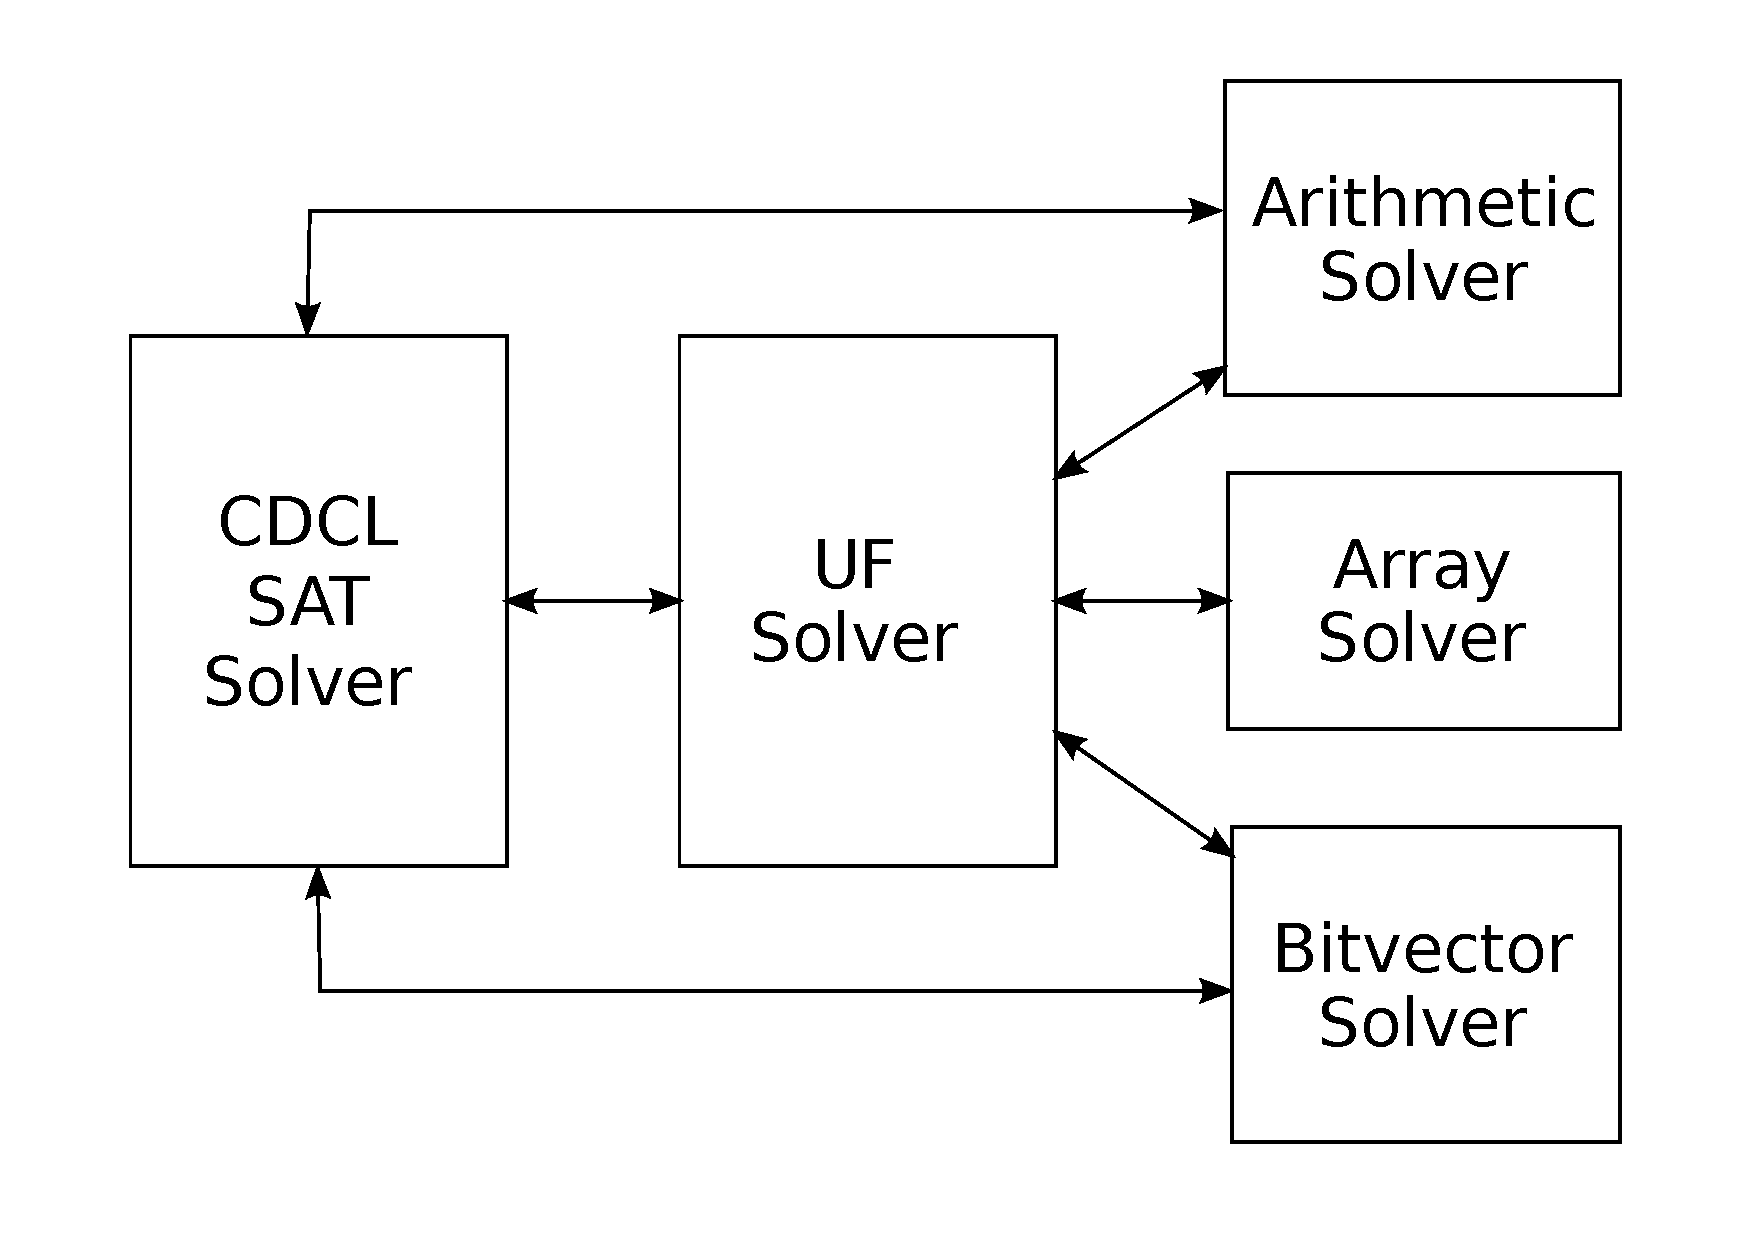
\includegraphics[width=10cm]{yices2-arch}
\end{center}
\caption{Solver Components}
\label{solver-architecture}
\end{figure}


It   is    possible   to   remove   some   of    the   components   of
Figure~\ref{solver-architecture} to  build simpler and  more efficient
solvers that are specialized for  classes of formulas.  For example, a
solver  for pure  arithmetic can  be built  by directly  attaching the
arithmetic solver to  the CDCL SAT solver.  Similarly,  Yices~2 can be
specialized  for pure  bitvector problems,  or for  problems combining
uninterpreted  functions,  arrays,  and  bitvectors (by  removing  the
arithmetic solver).

Yices~2 combines several theory solvers using the Nelson-Oppen
method~\cite{NelsonOppen79}.  The UF solver is essential for this
purpose; it coordinates the different theory solvers and ensures
global consistency. The other solvers (for arithmetic, arrays, and
bitvectors) communicate only with the central UF solver and never
directly with each other.  This property considerably simplifies the
design and implementation of theory solvers.  More details on the
theory-combination method implemented by Yices are given in a tool
paper~\cite{Dutertre:cav2014}.


\section{Context Configurations}
\label{features}

A context can be configured to use different solvers and to support
different usage scenarios. The basic operations on a context
include:
\begin{itemize}
\item asserting one or more formulas
\item checking satisfiability of the set of assertions
\item building a model if the assertions are satisfiable
\end{itemize}
Optionally, a context can support addition and removal of assertions
using a push/pop mechanism.  In this case, the context maintains a
stack of assertions organized in successive levels.  The push
operation starts a new level, and the pop operation removes all
assertions at the top level.  Thus, push can be thought as setting a
backtracking point and pop restores the context state to a previous
backtracking point.

Support for  push and pop induces  some overhead and  may disable some
preprocessing and  simplification of assertions. In some  cases, it is
then desirable to  use a context without support for  push and pop, in
order to get  higher performance. Yices~2 allows users  to control the
set of  features supported by a  context by selecting  a specific {\em
  operating mode\/}.
\begin{itemize}
\item The simplest mode is {\em one-shot\/}. In this mode, one can
  assert formulas then make a one call to the check operation.
  Assertions are not allowed after the call to check. This mode is the
  most efficient as Yices may apply powerful preprocessing and
  simplification (such as symmetry breaking~\cite{Deharbe+etal:2011}).
\item The next mode is {\em multi-checks\/}. In this mode, several calls
  to the check operation are allowed. One can assert formulas, call
  check, assert more formulas and call check again. This can be done
  as long as the context is satisfiable. Once check returns
  \texttt{unsat}, then no assertions can be added. This mode avoids
  the overhead of maintaining a stack of assertions.
\item The default mode is {\em push-pop\/}. In this mode, a context
  supports the push and pop operations. Assertions are organized in a
  stack as explained previously.
\item The last mode is {\em interactive\/}. This mode provides the
  same functionalities as {\em push-pop\/} but the context is
  configured to recover gracefully when a check operation times out or
  is interrupted.
\end{itemize}


\section{MCSAT}
\label{mcsat}

Since version~2.4.0, Yices includes another solver that uses a
different approach and architecture. This new solver is based on the
Model Constructing Satisfiability Calculus (MCSAT), and it is
currently dedicated to quantifier-free nonlinear real arithmetic. The
theory and implementation of MCSAT is discussed in several
publications~\cite{Jovanovic-etal:MCSATb:2013,deMouraJovanovic:MCSAT:2013}.
Currently, this solver can process input written in the SMT-LIB~2.0 or
Yices notations. The MCSAT solver is required for nonlinear
arithmetic, but it also supports other theories such as uninterpreted
functions or bitvectors.


\section{Third-Party SAT Solvers}

In Yices 2.6.2, we have added support for using third-party Boolean
satisfiability solvers. Such solvers are optional but can provide
significant performance improvements on bit-vector problems. Use of
these SAT solvers is enabled by a command-line option and is currently
restricted to non-incremental QF\_BV problems. If an external solver
is selected, Yices will perform ``bit blasting,'' that is, convert the
problem to an equisatisfiable SAT problem in conjunctive normal form
(CNF) and use the third-party solver to check satisfiability of this
CNF formula.




%%%%%%%%%%%%%%%%%%%%%%%%%%%%%%%%%
\chapter{Yices Tool}
\label{yices-shell}
%%%%%%%%%%%%%%%%%%%%%%%%%%%%%%%%%

The Yices~2 distribution includes  a tool for processing input written
in  the Yices~2  language.  This  tool is  called  \texttt{yices} (or
\texttt{yices.exe}  in  the Windows  and  Cygwin distributions).   The
syntax  and  the  set  of  commands supported  by  \texttt{yices}  are
explained  in  the file  \texttt{doc/YICES-LANGUAGE}  included in  the
distribution. Several example specifications  are also included in the
\texttt{examples} directory.

\begin{figure}[ht]
\begin{footnotesize}
\begin{verbatim}
  (define-type BV (bitvector 32))

  (define a::BV)
  (define b::BV)
  (define c::BV (mk-bv 32 1008832))
  (define d::BV)

  (assert (= a (bv-or (bv-and (mk-bv 32 255)
                              (bv-not (bv-or b (bv-not c))))
                      (bv-and c (bv-xor d (mk-bv 32 1023))))))

  (check)

  (show-model)
  (eval a)
  (eval b)
  (eval c)
  (eval d)
\end{verbatim}
\end{footnotesize}
\caption{Example Yices Script}
\label{example:bv_test2}
\end{figure}

\section{Example}

To      illustrate     the      tool     usage,      consider     file
\texttt{examples/bv\_test2.ys} shown in Figure~\ref{example:bv_test2}.
The  first line  defines  a  type called  \texttt{BV}.  In this  case,
\texttt{BV} is  a synonym for bitvectors  of size 32. Then  four terms
are  declared of  type \texttt{BV}.   The three  constants \texttt{a},
\texttt{b},  and \texttt{d}  are  uninterpreted,  while \texttt{c}  is
defined as  the bitvector representation  of the integer  1008832. The
next line of the file is  an assertion expressing a constraint between
\texttt{a},  \texttt{b},  \texttt{c},   and  \texttt{d}.  The  command
\texttt{(check)} checks whether the assertion is satisfiable. Since it
is, command  \texttt{(show-model)} asks for  a satisfying model  to be
displayed. The  next commands ask for  the value of four  terms in the
model.


\medskip\noindent
To run \texttt{yices} on this input file, just type
\begin{small}
\begin{lstlisting}[language=sh]
   yices examples/bv_test2.ys
\end{lstlisting}
\end{small}
The tool will output something like this:
\begin{small}
\begin{verbatim}
      sat
      (= d 0b00000000000000000000000000000000)
      (= b 0b00000000000000000000000000000000)
      (= a 0b00000000000000000000000011000000)

      0b00000000000000000000000011000000
      0b00000000000000000000000000000000
      0b00000000000011110110010011000000
      0b00000000000000000000000000000000
\end{verbatim}
\end{small}
The result of the \texttt{(check)}  command is shown on the first line
(i.e., \texttt{sat}  for satisfiable). The  next three lines  show the
model as  an assignment to  the three uninterpreted  terms \texttt{a},
\texttt{b},  and \texttt{d}.  Then,  the tool  displays one  bitvector
constant for each of the \texttt{(eval ...)} command.

\medskip\noindent
Since  this  example  contains  only  terms and  constructs  from  the
bitvector  theory,  we  could  specify logic  \texttt{QF\_BV}  on  the
command line as follows:
\begin{small}
\begin{lstlisting}[language=sh]
   yices --logic=QF_BV examples/bv_test2.ys
\end{lstlisting}
\end{small}
Since the file does not use \texttt{push} and \texttt{pop}, and it
contains only one call to \texttt{(check)}, we can select the mode
\texttt{one-shot}:
\begin{small}
\begin{lstlisting}[language=sh]
   yices --logic=QF_BV --mode=one-shot examples/bv_test2.ys
\end{lstlisting}
\end{small}
`To get a more detailed output, we can give a non-zero verbosity level:
\begin{small}
\begin{lstlisting}[language=sh]
   yices --verbosity=4 examples/bv_test2.ys
\end{lstlisting}
\end{small}

\section{Exists/Forall Problems}

\begin{figure}
\begin{footnotesize}
\begin{verbatim}
    (define x::real)

    (assert
      (forall (y::real)
         (=> (and (< (* -1 y) 0) (< (+ -10 y) 0))
             (< (+ -7 (* -2 x) y) 0))))

    (ef-solve)
    (show-model)
\end{verbatim}
\end{footnotesize}
\caption{Example Exists/Forall Problem}
\label{example:ef}
\end{figure}

Yices can solve a restricted class of quantified problems, known as
\emph{exists/forall problems\/}. As the name indicates, such
problems are of the following general form:
$$\exists x_1,\ldots,x_n:\forall
y_1,\ldots,y_m: P(x_1,\ldots,x_n,y_1,\ldots,y_m).$$ In many
applications, the goal to find values $a_1,\ldots,a_n$ for the
existentially quantified variables $x_1,\ldots,x_n$ such that the
following formula $$\forall
y_1,\ldots,y_m: P(a_1,\ldots,a_n,y_1\ldots,y_m)$$ is valid.

\medskip\noindent
Yices can solve such problems when the quantified variables
$x_1,\ldots,x_n$ and $y_1,\ldots,y_m$ either have finite type or are
real variables. The algorithm implemented in Yices and an example
application are described in~\cite{Gascon+etal:fmcad2014}.

\medskip\noindent Figure~\ref{example:ef} shows how exists/forall
problems are specified in the Yices language. Global declarations,
such as the uninterpreted constant \texttt{x} in the figure,
correspond to the existential variables.  Constraints are then stated
as assertions be of the form \texttt{(forall (y ...) P)} where
\texttt{y ...} are universal variables. It is allowed to have several
assertions of this form, as well as quantifier-free constraints on the
global variables.

\medskip\noindent
The command \texttt{(ef-solve)} invokes the exists/forall solver. This
commands is similar to \texttt{(check)}. It reports \texttt{sat} if
the problem is satisfiable, \texttt{unsat} if it is not, or
\texttt{unknown} if the solver does not terminate within a fixed
number of iterations. If \texttt{(ef-solve)} returns \texttt{sat},
then we can display the solution it has found using \texttt{(show-model)}.
This is illustrated in Figure~\ref{example:ef}.

\medskip\noindent
To run \texttt{yices} on this example, we must give option
\texttt{--mode=ef} on the command line:
\begin{small}
\begin{lstlisting}[language=sh,deletekeywords={test}]
   yices --mode=ef test.ys
\end{lstlisting}
\end{small}
This will produce the following output:
\begin{small}
\begin{verbatim}
      sat
      (= x 2)
\end{verbatim}
\end{small}
The first line is the result of \texttt{(ef-solve)}. The second line
is the model, which just shows the value of the global variable
\texttt{x}.

\medskip\noindent
As previously, we can get more detailed output by increasing the verbosity:
\begin{small}
\begin{lstlisting}[language=sh]
   yices --mode=ef --verbosity=5 test.ys
\end{lstlisting}
\end{small}
It is also possible to specify a logic on the command-line.

\section{Unsat Cores}

Since version 2.6.1, the Yices tool can produce unsat cores. This
feature comes in two flavors, as in SMT-LIB~2.6.

\subsection{Labeled Assertions}

The first method is illustrated in
Figure~\ref{example:labeled-assertions}. One gives labels to assertions and
command \texttt{(show-unsat-core)} displays an unsat core when a call
to \texttt{(check)} returns \texttt{unsat}.  The labels can be any
symbols; there is a separate name space for these labels.

\begin{figure}[h]
\begin{footnotesize}
\begin{verbatim}
    (define x::real)

    (assert (>= x 0))   ;; regular assertion
    (assert (> x 3) A)  ;; labeled assertion: A is the label
    (assert (< x 3) B)  ;; labeled assertion
    (assert (= x 3) C)  ;; another labeled assertion
    (check)             ;; will return unsat
    (show-unsat-core)   ;; display unsat core
\end{verbatim}
\end{footnotesize}
\caption{Unsat cores using labeled assertions}
\label{example:labeled-assertions}
\end{figure}


\subsection{Check With Assumptions}

The second method uses command \texttt{(check-assuming ...)}, a
variant of the \texttt{(check)} command that takes a list of
assumptions as arguments.  This is illustrated in
Figure~\ref{example:check-assuming}. An assumption is a restricted
form of terms. It can be either \texttt{<name>} or \texttt{(not
  <name>)}, where \texttt{<name>} is the name of a Boolean term.  If
\texttt{(check-assuming)} returns \texttt{unsat}, then one can get an
unsat core using \texttt{(show-unsat-assumptions)}. This command shows
a subset of the assumptions that are inconsistent with the context.

\begin{figure}[h]
\begin{footnotesize}
\begin{verbatim}
    (define x::real)
    (define A::bool (> x 3))
    (define B::bool (> x 2))
    (define C::bool (> x 4))

    (assert (and (>= x 0) <= x 5)) ;; regular assertion
    (check-assuming A (not B) C)   ;; will return unsat
    (show-unsat-assumptions)       ;; unsat core: (A (not B))
\end{verbatim}
\end{footnotesize}
\caption{Check with assumptions}
\label{example:check-assuming}
\end{figure}





\section{Tool Invocation}

Yices is invoked on an input file by typing
\begin{lstlisting}[language=sh]
   yices [option] <filename>
\end{lstlisting}
If no \texttt{<filename>} is given, \texttt{yices} will run in
interactive mode and will read the standard input. The following
options are supported.
\begin{options}
\item[--logic=<name>] Select an SMT-LIB logic.

  The \texttt{<name>} must either be an SMT-LIB logic name such as
  \texttt{QF\_UFLIA} or the special name \texttt{NONE}.

  Yices recognizes the logics defined at \url{http://www.smtlib.org}
  (as of July 2014).  Option \texttt{--logic=NONE} configures
  \texttt{yices} for propositional logic.

  By default---that is, if no logic is given---\texttt{yices} includes
  all the  theory solvers described in  Section~\ref{solvers}. In this
  default  configuration, \texttt{yices}  supports  linear arithmetic,
  bitvectors,  uninterpreted  functions, and  arrays.  If  a logic  is
  specified, \texttt{yices}  uses a specialized  solver or combination
  of  solvers that is  appropriate for  the given  logic. Some  of the
  search parameters will also be set  to values that seem to work well
  for  this logic (based  on extensive  benchmarking). All  the search
  parameters  can  also be  modified  individually  using the  command
  \texttt{(set-param ...)}.

  If  option  \texttt{--logic=NONE}   is  given,  then  \texttt{yices}
  includes no  theory solvers  at all. All  assertions must  be purely
  propositional (i.e., involve only Boolean terms).

  If the selected logic includes nonlinear arithmetic (e.g.,
  \texttt{--logic=QF\_UFNRA}), then \texttt{yices} will automatically
  select the MCSAT solver. To force use of the MCSAT solver on logics
  that do not require it, use command-line option \texttt{--mcsat}.

\item[--arith-solver=<solver>] Select one of the possible arithmetic solvers.\\[1mm]
  \texttt{<solver>}     must    be     one     of    \texttt{simplex},
  \texttt{floyd-warshall}, or \texttt{auto}.

  If  the  logic is  \texttt{QF\_IDL}  (integer  difference logic)  or
  \texttt{QF\_RDL} (real  difference logic),  then this option  can be
  used   to  select   the  arithmetic   solver:  either   the  generic
  Simplex-based  solver   or  a   specialized  solver  based   on  the
  Floyd-Warshall algorithm.  If option \texttt{--arith-solver=auto} is
  given, then  the arithmetic solver is  determined automatically; the
  default is \texttt{auto}.

  This option has no effect  for logics other than \texttt{QF\_IDL} or
  \texttt{QF\_RDL}.

\item[--mode=<mode>] Select solver features.\\[1mm]
  \texttt{<mode>} can be \texttt{one-shot}, \texttt{multi-checks},
  \texttt{push-pop}, \texttt{interactive}, or \texttt{ef}.

  The mode \texttt{ef} enables the exists/forall solver. In this mode,
  Yices can solve problems  with universally quantified variables. The
  command  \texttt{(ef-solve)}  can be  used  for  a single  block  of
  assertions.    No  assertions   are  allowed   after  the   call  to
  \texttt{(ef-solve)}.

  The other four modes select the set of functionalities supported by
  the solver as follows:
  \begin{itemize}
  \item   \texttt{one-shot}:   no   assertions   are   allowed   after
    the \texttt{(check)} command. In this mode, \texttt{yices} can
    check satisfiability of a single block of assertions and possibly
    build a model if the assertions are satisfiable.
  \item \texttt{multi-checks}: several  calls to \texttt{(assert)} and
    \texttt{(check)} are allowed.
  \item \texttt{push-pop}: like \texttt{multi-checks} but with support
    for   adding   and   retracting   assertions  via   the   commands
    \texttt{(push)} and \texttt{(pop)}.
  \item  \texttt{interactive}:  supports  the  same  features  as  the
    \texttt{push-pop}  mode,  but  with   a  different  behavior  when
    \texttt{(check)} is interrupted.
  \end{itemize}
  In  the  first  two  modes, \texttt{yices}  employs  more  aggressive
  simplifications when processing assertions;  this can lead to better
  performance on some problems.

  Unsat cores and checks with assumptions are not supported in mode
  \texttt{one-shot}.

  In interactive mode,  the solver context is saved  before every call
  to  \texttt{(check)}  and  it  is restored  if  \texttt{(check)}  is
  interrupted. This introduces some  overhead, but the solver recovers
  gracefully if  \texttt{(check)} is interrupted or times  out. In the
  non-interactive modes, the solver exits after the first interruption
  or timeout.

  The default mode is \texttt{push-pop} if a file name is given on the
  command line. If  not input file is given, then  the default mode is
  \texttt{interactive} and the solver reads standard input.

  Mode \texttt{one-shot} is required to use the Floyd-Warshall solvers.

\item[--mcsat] Force use the MCSAT solver.

  This option forces \texttt{yices} to use the MCSAT solver instead of
  the default CDCL($T$) solver. By default, MCSAT is used only if the
  logic includes non-linear arithmetic. Using option \texttt{--mcsat}
  selects the MCSAT solver on other logics. For example, this can be
  used to use the MCSAT solver on bitvector problems.

\item[--print-success] Print \texttt{ok} after every command that would
  otherwise execute silently.

  Many commands are executed silently by \texttt{yices} (i.e., they
  produce no output). This can be a problem for tools that interact
  with \texttt{yices} via pipes or files. Option
  \texttt{--print-success} modifies this behavior. With this option,
  \texttt{yices} will print \texttt{ok} on its standard output when a
  command successfully executes.

\item[--version, -V] Display version information then exit.

  This  displays the  Yices version  number,  the version  of the  GMP
  library  linked with  Yices, and  information about  build date  and
  platform. For example,  here is the output for  Yices~2.2.0 built on
  MacOS~X
  \begin{small}
  \begin{verbatim}
     Yices 2.2.0
     Copyright SRI International.
     Linked with GMP 5.1.3
     Copyright Free Software Foundation, Inc.
     Build date: 2013-12-21
     Platform: x86_64-apple-darwin13.0.2 (release)
  \end{verbatim}
  \end{small}
  \vspace*{-1em}
  If you ever have to report a bug, please include this version information
  in your bug report.

\item[--help, -h] Print a summary of options

\item[--verbosity=<level>, -v <level>] Run in verbose mode.
\end{options}
As indicated in this list, some options can be given either in a long
form (like \texttt{--verbosity=4}) or in an equivalent short from (like
\texttt{-v 4}). In all cases the long and short forms are equivalent.

\section{Input Language}

The   syntax  of   the   Yices  input   language   is  summarized   in
Figures~\ref{syntax:commands} to~\ref{syntax:expressions}.


\begin{figure}
\begin{small}
\begin{verbatim}
   <command>  ::=
              ( define-type <symbol> )
            | ( define-type <symbol> <typedef> )
            | ( define <symbol> :: <type> )
            | ( define <symbol> :: <type> <expression> )
            | ( assert <expression> )
            | ( assert <expression> <symbol> )
            | ( exit )
            | ( check )
            | ( check-assuming <assumption-list> )
            | ( push )
            | ( pop )
            | ( reset )
            | ( show-model )
            | ( eval <expression> )
            | ( echo <string> )
            | ( include <string> )
            | ( set-param <symbol> <immediate-value> )
            | ( show-param <symbol> )
            | ( show-params )
            | ( show-stats )
            | ( reset-stats )
            | ( set-timeout <number> )
            | ( show-timeout )
            | ( dump-context )
            | ( help )
            | ( help <symbol> )
            | ( help <string> )
            | ( ef-solve )
            | ( export-to-dimacs <string> )
            | ( show-implicant )
            | ( show-unsat-core )
            | ( show-unsat-assumptions )
            | ( show-reduced-model )
            | EOS

\end{verbatim}
\end{small}
\caption{Yices Syntax: Commands}
\label{syntax:commands}
\end{figure}

\begin{figure}
\begin{small}
\begin{verbatim}
   <immediate-value> ::=
              true
            | false
            | <number>
            | <symbol>

   <number> ::= <rational> | <float>

   <assumption-list> ::=
            |
            | <assumption> <assumption-list>

   <assumption> ::=
            | <symbol>
            | ( not <symbol> )

\end{verbatim}
\end{small}
\caption{Yices Syntax: Command Arguments}
\end{figure}

\begin{figure}
\begin{small}
\begin{verbatim}
   <typedef> ::=
              <type>
            | ( scalar <symbol> ... <symbol> )

   <type> ::=
              <symbol>
            | ( tuple <type> ... <type> )
            | ( -> <type> ... <type> <type> )
            | ( bitvector <rational> )
            | int
            | bool
            | real
\end{verbatim}
\end{small}
\caption{Yices Syntax: Types}
\label{syntax:types}
\end{figure}

\begin{figure}
\begin{small}
\begin{verbatim}
   <expr> ::=
              true
            | false
            | <symbol>
            | <rational>
            | <float>
            | <binary bv>
            | <hexa bv>
            | ( forall ( <var_decl> ... <var_decl> ) <expr> )
            | ( exists ( <var_decl> ... <var_decl> ) <expr> )
            | ( lambda ( <var_decl> ... <var_decl> ) <expr> )
            | ( let ( <binding> ... <binding> ) <expr> )
            | ( update <expr> ( <expr> ... <expr> ) <expr> )
            | ( <function> <expr> ... <expr> )

   <function> ::=
              <function-keyword>
            | <expr>

   <var_decl> ::= <symbol> :: <type>

   <binding> ::= ( <symbol> <expr> )
\end{verbatim}
\end{small}
\caption{Yices Syntax: Expressions}
\label{syntax:expressions}
\end{figure}

\subsection{Lexical  Elements}

\subsubsection*{Comments}

Input  files  may contain  comments,  which  start  with a  semi-colon
\texttt{`;'} and extend to the end of the line.

\subsubsection*{Strings}

Strings  are similar to  strings in  C. They  are delimited  by double
quotes \texttt{"} and may contain escaped characters:
\begin{itemize}
\item     The     characters     \texttt{\textbackslash     n}     and
  \texttt{\textbackslash   t}  are  replaced   by  newline   and  tab,
  respectively.
\item The character \texttt{\textbackslash}  followed by at most three
  octal digits  (i.e., from \texttt{0}  to \texttt{7}) is  replaced by
  the character whose ASCII code is the octal number.
\item In  all other cases, \texttt{\textbackslash  <char>} is replaced
  by  \texttt{<char>} (including  if \texttt{<char>}  is a  newline or
  \texttt{\textbackslash}).
\item A  newline cannot  occur inside the  string, unless  preceded by
  \texttt{\textbackslash}.
\end{itemize}

\subsubsection*{Numerical Constants}

Numerical  constants  can  be   written  as  decimal  integers  (e.g.,
\texttt{44} or \texttt{-3}), rational (e.g., \texttt{-1/3}), or using a
floating-point  notation  (e.g.,  \texttt{0.07} or  \texttt{-1.2e+2}).
Positive  constants can start  with an  optional \texttt{+}  sign. For
example \texttt{+4} and \texttt{4} denote the same number.


\subsubsection*{Bitvector Constants}

Bitvector constants can be written in a binary format using the prefix
\texttt{0b}  or  in  hexadecimal  using the  prefix  \texttt{0x}.  For
example, the expressions  \texttt{0b01010101} and \texttt{0x55} denote
the same bitvector constant of eight bits.

\subsubsection*{Symbols}

A  symbol  is   any  character  string  that's  not   a  keyword  (see
Table~\ref{syntax:keywords}) and doesn't start  with a digit, a space,
or   one  of  the   characters  \texttt{(},   \texttt{)},  \texttt{;},
\texttt{:}, and  \texttt{"}. If the  first character is  \texttt{+} or
\texttt{-}, then it must not be  followed by a digit. Symbols end by a
space, or by any of the characters \texttt{(}, \texttt{)}, \texttt{;},
\texttt{:}, or \texttt{"}. Here are some examples:
\begin{small}
\begin{verbatim}
   a_symbol __another_one  X123  &&&  +z203  t\12
\end{verbatim}
\end{small}
All   the   predefined   keywords    and   symbols   are   listed   in
Table~\ref{syntax:keywords}.

\begin{table}
\begin{small}
\begin{center}
\begin{tt}
\begin{tabular}{|p{3.4cm}|p{3.4cm}|p{4.7cm}|}
\hline
* & + & - \\
-> & / & /= \\
< & <= & <=> \\
 = & => & > \\
>= & \verb|^| & abs \\
and & assert & bit \\
bitvector & bool & bool-to-bv \\
bv-add & bv-and & bv-ashift-right\\
bv-ashr & bv-comp & bv-concat \\
bv-div  & bv-extract & bv-ge \\
bv-gt  & bv-le & bv-lshr \\
bv-lt  & bv-mul & bv-nand \\
bv-neg & bv-nor & bv-not\\
bv-or  & bv-pow & bv-redand \\
bv-redor & bv-rem & bv-repeat \\
bv-rotate-left & bv-rotate-right & bv-sdiv \\
bv-sge & bv-sgt & bv-shift-left0 \\
bv-shift-left1 & bv-shift-right0 & bv-shift-right1 \\
bv-shl & bv-sign-extend & bv-sle \\
bv-slt & bv-smod & bv-srem \\
bv-sub & bv-xnor & bv-xor \\
bv-zero-extend & ceil & check \\
define & define-type & distinct \\
div & divides & dump-context \\
echo  & ef-solve & eval \\
exists & exit & export-to-dimacs \\
false & floor & forall \\
help & if & include \\
int & is-int & ite \\
lambda & let & mk-bv \\
mk-tuple & mod & not \\
or & pop & push \\
real & reset & reset-stats \\
scalar & select & set-param \\
set-timeout & show-implicant & show-model \\
show-param & show-params & show-reduced-model \\
show-stats & show-unsat-core & show-unsat-assumptions \\
true & tuple & tuple-update \\
update & xor &  \\
\hline
\end{tabular}
\end{tt}
\end{center}
\end{small}
\caption{Keywords and predefined symbols}
\label{syntax:keywords}
\end{table}


\subsection{Declarations}
\label{declarations}

A declaration either introduces a new type or term or gives a name to
an existing type or term. Yices uses different name spaces for types
and terms. It is then permitted to use the same name for a type and
for a term.


\subsubsection*{Type Declaration}

A type declaration is a command of the following two forms.
\begin{small}
\begin{verbatim}
   (define-type name)
   (define-type name type)
\end{verbatim}
\end{small}
The fist form creates a new uninterpreted type called
\texttt{name}. The second form gives a \texttt{name} to an
existing \texttt{type}. After this definition, every occurrence of
\texttt{name} refers to \texttt{type}. A variant of this second
form is used to define scalar types. In these two commands,
\texttt{name} must be a symbol that's not already used as a type
name.


\subsubsection*{Term Declaration}

A term is declared using one for the following two commands.
\begin{small}
\begin{verbatim}
   (define name :: type)
   (define name :: type term)
\end{verbatim}
\end{small}
The first form declares a new uninterpreted term of the given
\texttt{type}.  The second form assigns a \texttt{name} to the
given \texttt{term}, which must be of type \texttt{type}. The
\texttt{name} must be a symbol that's not already used as a term
name.



\subsection{Types}

Yices includes a few predefined types for arithmetic and
bitvectors. One can extend the set of atomic types by creating
uninterpreted and scalar types. In addition to the atomic types, Yices
provides constructors for tuple and function types. More details about
types and subtyping are given in Section~\ref{type-system}.

\subsubsection*{Predefined Types}

The predefined  types are \texttt{bool},  \texttt{int}, \texttt{real},
and  \texttt{(bitvector  k)} where  $k$  is  a  positive integer.  For
example a bit-vector variable \texttt{b}  of 32 bits is declared using
the command
\begin{small}
\begin{verbatim}
   (define b::(bitvector 32))
\end{verbatim}
\end{small}
The number of bits must be positive so \texttt{(bitvector 0)} is not a
valid  type.   There  is  also  a hard-coded  limit  on  the  size  of
bitvectors (namely, $2^{28}  - 1$).  Of course, this  is a theoretical
limit; the solver will most likely run out of memory if you attempt to
use bitvectors that are that large.

\subsubsection*{Uninterpreted Types}

A new uninterpreted type T can be introduced using the command
\begin{small}
\begin{verbatim}
   (define-type T)
\end{verbatim}
\end{small}
This command  will succeed provided  \texttt{T} is a fresh  type name,
that is, if there is no existing type called \texttt{T}.  As explained
in Section~\ref{type-system}, an uninterpreted type denotes a nonempty
collection  of  objects.   There   is  no  cardinality  constraint  on
\texttt{T}, except that \texttt{T} is not empty.

\subsubsection*{Scalar Type}

A scalar type is defined by enumerating its elements. For example, the
following declaration
\begin{small}
\begin{verbatim}
   (define-type P (scalar A B C))
\end{verbatim}
\end{small}
defines a  new scalar type  called \texttt{P} that contains  the three
distinct  constants  \texttt{A}, \texttt{B},  and  \texttt{C}. Such  a
declaration  is valid  provided \texttt{P}  is a  fresh type  name and
\texttt{A}, \texttt{B}, and \texttt{C} are all fresh term names.

\medskip\noindent The enumeration must include at least one element,
but  singleton   types  are   allowed.  For  example,   the  following
declaration is valid.
\begin{small}
\begin{verbatim}
   (define-type Unit (scalar One))
\end{verbatim}
\end{small}
It introduces a  new type \texttt{Unit} of cardinality  one, and which
contains \texttt{One}  as its unique  element. Thus, any term  of type
\texttt{Unit} is known to be equal to \texttt{One}.


\subsubsection*{Tuple Types}

A tuple  type is written \texttt{(tuple tau\_1  ... tau\_n)} where
\texttt{tau\_i} is a type. For example, the type of pairs of integer
can be declared as follows:
\begin{small}
\begin{verbatim}
   (define-type Pairs (tuple int int))
\end{verbatim}
\end{small}
Then one can declare an uninterpreted constant \texttt{x} of this type
as follows
\begin{small}
\begin{verbatim}
   (define x::Pairs)
\end{verbatim}
\end{small}
This is equivalent to the declaration
\begin{small}
\begin{verbatim}
   (define x::(tuple int int))
\end{verbatim}
\end{small}

\medskip\noindent   Tuple  types   with  a   single   component  are
allowed. For example, the following declaration is legal.
\begin{small}
\begin{verbatim}
   (define-type T (tuple bool))
\end{verbatim}
\end{small}

\subsubsection*{Function Types}

A function type is written \texttt{(-> tau\_1 ...  tau\_n
  sigma)}, where $n$ is positive, and the \texttt{tau\_i}s and
\texttt{sigma} are types.  The types \texttt{tau\_1}, $\ldots$,
\texttt{tau\_n} define the domain of the function type, and
\texttt{sigma} is the range.  For example, a function defined over
the integers and that returns a Boolean can be declared as follows:
\begin{small}
\begin{verbatim}
   (define f::(-> int bool))
\end{verbatim}
\end{small}

\medskip\noindent Yices does not  have a distinct type construct for
arrays. In Yices, arrays are the same as functions.


\subsection{Terms}

Yices uses a Lisp-like syntax. For example, the polynomial $x + 3y +
z$ is written
\begin{small}
\begin{verbatim}
       (+ x (* 3 y) z)
\end{verbatim}
\end{small}
In general, all associative operations can take one, two, or more
arguments. For example, one can write
\begin{small}
\begin{verbatim}
      (or A)    (or A B)    (or A B C D)
\end{verbatim}
\end{small}
since \texttt{or} is associative.


\subsubsection*{If-Then-Else}

Yices provides an if-then-else construct that applies to any type.  An
if-then-else term can be written using either one of the two following
forms
\begin{small}
\begin{verbatim}
     (ite c t1 t2)     (if  c t1 t2)
\end{verbatim}
\end{small}
Both forms are equivalent and just mean ``if \texttt{c} then
\texttt{t1} else \texttt{t2}.''  The condition \texttt{c} must
be a Boolean term, and the two terms \texttt{t1} and \texttt{t2}
must have compatible types. If \texttt{t1} and \texttt{t2} have
the same type $\tau$ then \texttt{(ite c t1 t2)} also has type
$\tau$.  Otherwise, as explained in Section~\ref{type-system}, the
type of \texttt{(if c t1 t2)} is the minimal supertype of
\texttt{t1} and \texttt{t2}.  For example, if \texttt{t1} has
type \texttt{int} and \texttt{t2} has type \texttt{real}, then
\texttt{(ite c t1 t2)} has type \texttt{real}.

\subsubsection*{Equalities and Disequalities}

Equalities and disequalities are written as follows
\begin{small}
\begin{verbatim}
     (=  t1 t2)        (/= t1 t2)
\end{verbatim}
\end{small}
where \texttt{t1} and \texttt{t2} are two terms of compatible
types. These operators are binary. Unlike SMT-LIB~2, Yices does not
support constraints such as \texttt{(= x y z t u)}. On the other hand,
Yices includes an $n$-ary \texttt{distinct} operator that generalizes
disequality.

%% \pagebreak
\medskip\noindent
The Boolean term
\begin{small}
\begin{verbatim}
   (distinct t_1 .... t_n )
\end{verbatim}
\end{small}
is true if \texttt{t\_1}, \ldots, \texttt{t\_n} are all different
from each other. The terms \texttt{t\_1} to \texttt{t\_n} must all
have compatible types.  There must be at least two arguments. The
expression \texttt{(distinct a b)} means the same thing as \texttt{(/= a
  b)}.

\subsubsection*{Boolean Operators}

\begin{table}[h]
\begin{small}
\begin{center}
\begin{tabular}{|p{2cm}|p{2cm}|}
\hline
\texttt{true} & \texttt{false} \\
\texttt{and} & \texttt{or}  \\
\texttt{not} & \texttt{xor}  \\
\texttt{<=>} & \texttt{=>}  \\
\hline
\end{tabular}
\end{center}
\end{small}
\caption{Boolean Constants and Operators}
\label{Boolean-Operators}
\end{table}

\noindent
The usual Boolean constants and functions are available. They are
listed in Table~\ref{Boolean-Operators}.  The associative and
commutative operators \texttt{or}, \texttt{and}, and \texttt{xor} can
take any number of arguments. The equivalence (\texttt{<=>}) and
implication (\texttt{=>}) operators take exactly two arguments.

\medskip\noindent
One can also use the equality and disequality operators
with Boolean terms. If \texttt{t1} and \texttt{t2} are Boolean
then \texttt{(= t1 t2)} is the same as \texttt{(<=> t1 t2)},
and \texttt{(/= t1 t2)} is the same as \texttt{(xor t1 t2)}.

\subsubsection*{Basic Arithmetic}

\begin{table}[h]
\begin{small}
\begin{center}
\begin{tabular}{|p{4cm}|l|c|}
\hline
Syntax & \multicolumn{2}{|c|}{Meaning} \\
\hline
\texttt{(+ a1 ... a\_n)} & sum & $a_1 + \ldots + a_n$ \\
\texttt{(* a1 ... a\_n)} & product & $a_1 \times \ldots \times a_n$ \\
\texttt{(- a)} & opposite & $-a$\\
\texttt{(- a1 a2 ... a\_n)} & difference &  $a_1 - a_2 - \ldots - a_n$ \\
\texttt{(\char`\^\  a k)} & exponentiation & $a^k$ \\
\texttt{(/ a c)} & division & $a/c$ \\
\hline
\texttt{(<= a1 a2)} & inequality & $a_1 \leq a_2$\\
\texttt{(>= a1 a2)} & inequality & $a_1 \geq a_2$\\
\texttt{(< a1 a2)} & strict inequality & $a_1 < a_2$ \\
\texttt{(> a1 a2)} & strict inequality & $a_1 > a_2$ \\
\hline
\end{tabular}
\end{center}
\end{small}
\caption{Arithmetic Operations}
\label{Arithmetic-Operations}
\end{table}

Arithmetic constants can be written in decimal, as rationals, or using
the floating point notation. Internally, Yices uses exact rational
arithmetic and it represents all arithmetic constants as rationals.

\medskip\noindent
The usual arithmetic operations and comparison operators are
summarized in Table~\ref{Arithmetic-Operations}. One can freely mix
terms of real and integer types in all operations. The exponent $k$ in
\texttt{(\char`\^\ a k)} must be a non-negative integer constant. The
divisor \texttt{c} in \texttt{(/ a c)} must be a non-zero constant.


\medskip\noindent
The Yices language includes more than linear arithmetic, but this is
for future extensions. Currently, Yices does not include solvers for
non-linear arithmetic (cf. Section~\ref{solvers}).

\subsubsection*{Arithmetic Functions}

Other arithmetic operations defined in Yices are listed in Table~\ref{Arithmetic-Functions}.
The operations \texttt{abs}, \texttt{floor}, and \texttt{ceil} have the usual meaning:
\begin{itemize}
\item \texttt{(abs x)} is the absolute value of \texttt{x}.
\item \texttt{(floor x)} is the largest integer less than or equal to \texttt{x}.
\item \texttt{(ceil x)} is the smallest integer larger than or equal to \texttt{x}.
\end{itemize}
For integer division and modulo, Yices uses the SMT-LIB conventions (see
Section~\ref{arithmetic-general}), except that the divider \texttt{k}
must be a non-zero constant and that both \texttt{div} and
\texttt{mod} are defined over the reals, not just the integers.
Division by a non-constant term is not supported.

\medskip\noindent In the divisibility test \texttt{(divides k x)}, the
divider \texttt{k} must be a rational constant but it can be zero. The
term \texttt{x} can be any real. The atom \texttt{(divides k x)} is
true if there exists an integer $n\in\integers$ such that $\mathtt{x} = n
\mathtt{k}$.

\begin{table}[h]
\begin{small}
\begin{center}
\begin{tabular}{|p{3.4cm}|l|}
\hline Syntax & Meaning \\
\hline
\texttt{(abs x)} & absolute value \\
\texttt{(floor x)} & floor \\
\texttt{(ceil x)} & ceiling \\
\hline
\texttt{(div x k)} & integer division \\
\texttt{(mod x k)} & modulo \\
\texttt{(divides k x)} & divisibility test\\
\texttt{(is-int x)} & integrality test\\
\hline
\end{tabular}
\end{center}
\end{small}
\caption{Arithmetic Functions}
\label{Arithmetic-Functions}
\end{table}

\subsubsection*{Bitvectors Constants}

A bitvector constant can be written in binary or hexadecimal notation, as follows
\begin{small}
\begin{verbatim}
   0b0   0b1   0xFFFF    0xaaaa    0xC0C0D0D0
\end{verbatim}
\end{small}
In the binary notation, the number of bits in the constant is equal to
be number of binary digits. For example, the three terms
\begin{small}
\begin{verbatim}
   0b1   0b0001   0b00001
\end{verbatim}
\end{small}
denote distinct bitvector constants, of one, four, and five bits, respectively.
In the hexadecimal notation, the number of bits is equal to four times the number
of hexadecimal digit.

\medskip\noindent
One can also construct a bitvector constant using the expression:
\begin{small}
\begin{verbatim}
   (mk-bv size value)
\end{verbatim}
\end{small}
In this expression, both \texttt{size} and \texttt{value} must be
integer constants; \texttt{size} is the number of bits in the
bitvector constant and \texttt{value} is the decimal value of the
constant interpreted as a non-negative integer. The \texttt{size}
must then be positive, and the \texttt{value} must be
non-negative. If \texttt{value} is more than $2^{\mathtt{size}}$,
only the residue of \texttt{value} modulo $2^{\mathtt{size}}$ is
taken into account. For example, the expressions
\begin{small}
\begin{verbatim}
   (mk-bv 3 6)    (mk-bv 3 22)
\end{verbatim}
\end{small}
construct the same bitvector constant (whose binary representation is
\texttt{0b110}).

\subsubsection*{Bitvector Arithmetic}

\begin{table}
\begin{small}
\begin{center}
\begin{tabular}{|p{5cm}|l|}
\hline Syntax & Meaning \\
\hline
\texttt{(bv-add u1 ... u\_n)} & sum \\
\texttt{(bv-mul u1 ... u\_n)} & product \\
\texttt{(bv-sub u1 ... u\_n)} & subtraction \\
\texttt{(bv-neg u)} & 2s-complement \\
\texttt{(bv-pow u k)} & exponentiation \\
\hline
\texttt{(bv-not u)} & bitwise complement \\
\texttt{(bv-and u1 ... u\_n)} & bitwise and \\
\texttt{(bv-or u1 ... u\_n)} & bitwise or \\
\texttt{(bv-xor u1 ... u\_n)} & bitwise xor \\
\texttt{(bv-nand u1 ... u\_n)} & bitwise nand \\
\texttt{(bv-nor u1 ... u\_n)} & bitwise nor \\
\texttt{(bv-xnor u1 ... u\_n)} & bitwise xnor \\
\hline
\end{tabular}
\end{center}
\end{small}
\caption{Bitvector Operations (Arithmetic and Bitwise Logic)}
\label{bitvectors1}
\end{table}

Table~\ref{bitvectors1} lists all the arithmetic and bitwise
operators. All operators in this table take arguments that have the
same size and return a result of that size.  As usual, the associative
operators can take one, two, or more arguments. The \texttt{bv-sub}
operator takes at least two arguments. In \texttt{(bv-pow u k)},
the power $k$ must be a non-negative integer constant.

\medskip\noindent
The expression \texttt{(bv-xnor u1 ... u\_n)} is the same as
\texttt{(bv-not (bv-xor u1 ... u\_n))}.

\subsubsection*{Bitvector Shift and Rotate}

\begin{table}
\begin{small}
\begin{center}
\begin{tabular}{|p{5cm}|l|}
\hline
Syntax & Meaning \\
\hline
\texttt{(bv-shift-left0 u k)} & left shift, padding with 0\\
\texttt{(bv-shift-left1 u k)} & left shift, padding with 1\\
\texttt{(bv-shift-right0 u k)} & right shift, padding with 0\\
\texttt{(bv-shift-right1 u k)} & right shift, padding with 1\\
\texttt{(bv-ashift-right x k)} &  arithmetic shift by $k$ bits\\
\texttt{(bv-rotate-left x k)} & rotate by $k$ bits to the left\\
\texttt{(bv-rotate-right x k)} & rotate by $k$ bits to the right\\
\hline
\texttt{(bv-shl u v)} & left shift (padding with 0)\\
\texttt{(bv-lshr u v)} & logical right shift (padding with 0) \\
\texttt{(bv-ashr u v)} & arithmetic shift (padding with the sign bit)\\
\hline
\end{tabular}
\end{center}
\end{small}
\caption{Bitvector Operations (Shift and Rotate)}
\label{bitvectors2}
\end{table}

Table~\ref{bitvectors2} lists the shift and rotate operations. The
operations in the first seven rows shift a bitvector \texttt{u} by a
fixed number of bits $k$. If \texttt{u} is a bitvector of $n$ bits,
then $k$ must be an integer constant such that $0 \leq k \leq n$. The
\texttt{bv-shl}, \texttt{bv-lshr}, and \texttt{bv-ashr} operators
(last three rows of Table~\ref{bitvectors2}) take two bitvector
arguments \texttt{u} and \texttt{v}, which must be bitvectors of the
same size $n$. The shift operation is applied to \texttt{u} and the
value of \texttt{v}, interpreted as an unsigned integer in the range
$[0, 2^n-1]$, defines the shift amount. The semantics follows the
SMT-LIB standards: if \texttt{v}'s value is more than $n$ then the
padding bit is copied $n$ times.

\subsubsection*{Bitvector Structural Operations}

\begin{table}
\begin{small}
\begin{center}
\begin{tabular}{|p{5cm}|l|}
\hline
Syntax & Meaning \\
\hline
\texttt{(bv-extract i j u)} & subvector extraction \\
\texttt{(bv-concat u1 ... u\_n)} & concatenation \\
\texttt{(bv-repeat u k)} & repeated concatenation \\
\texttt{(bv-sign-extend u k)} & sign extension \\
\texttt{(bv-zero-extend u k)} & zero extension \\
\hline
\texttt{(bv-redor u)} & or-reduction \\
\texttt{(bv-redand u)} & and-reduction \\
\texttt{(bv-redcomp u v)} & equality reduction \\
\hline
\end{tabular}
\end{center}
\end{small}
\caption{Bitvector Operations (Structural Operators)}
\label{bitvectors3}
\end{table}

The operators in Table~\ref{bitvectors3} perform extraction,
concatenation, and other structural operations. The expression
\texttt{(bv-extract i j u)} is the segment of bitvector \texttt{u}
formed by taking bits $j, j+1, \ldots, i$. If \texttt{u} is a
bitvector of $n$ bits then the constants $i$ and $j$ must satisfy $0
\leq j \leq i \leq n-1$, and the result is a bitvector of $(i - j +
1)$ bits. For example, we have
\begin{small}
\begin{verbatim}
   (bv-extract 7 2 0b110110100) = 0b101101.
\end{verbatim}
\end{small}

\medskip\noindent
In \texttt{(bv-repeat u k)}, bitvector \texttt{u} is concatenated with
itself $k$ times. The integer constant $k$ must be positive. In the
sign and zero extension operators, vector \texttt{u} is extended by
adding $k$ bits (either zero or \texttt{u}'s sign bit copied $k$
times).  In these two operations, $k$ must be non-negative.

\medskip\noindent
The \texttt{bv-redor}, \texttt{bv-redand}, and \texttt{bv-redcomp}
operators produce a one-bit vector.  The term \texttt{(bv-redor u)} is
the or of \texttt{u}'s bits; it is equal to \texttt{0b0} if all bits
of \texttt{u} are zero, and to \texttt{0b1} otherwise. Similarly,
\texttt{(bv-redand u)} is the and of \texttt{u}'s bit; it is equal to
\texttt{0b1} if all bits of \texttt{u} are one and to \texttt{0b0}
otherwise. In \texttt{(bv-redcomp u v)}, the arguments \texttt{u} and
\texttt{v} must be two bitvectors of the same size. The operator
performs a one-to-one comparison of the bits of \texttt{u} and
\texttt{v} and returns either \texttt{0b1}, if \texttt{u} and
\texttt{v} are equal, or \texttt{0b0}, if \texttt{u} and \texttt{v}
are distinct.

\subsubsection*{Bitvector Division}

\begin{table}
\begin{small}
\begin{center}
\begin{tabular}{|p{3.3cm}|l|}
\hline
Syntax & Meaning \\
\hline
\texttt{(bv-div u v)} & quotient in unsigned division \\
\texttt{(bv-rem u v)} & remainder in unsigned division \\
\hline
\texttt{(bv-sdiv u v)} & quotient in signed division \\
\texttt{(bv-srem u v)} & remainder in signed division \\
\hline
\texttt{(bv-smod u v)} & remainder in signed division (rounding to $-\infty$)\\
\hline
\end{tabular}
\end{center}
\end{small}
\caption{Bitvector Operations (Divisions)}
\label{bitvectors4}
\end{table}

Table~\ref{bitvectors4} lists the division and remainder operators. In
this table, \texttt{u} and \texttt{v} must be two bitvectors of the
same size $n$.

\medskip\noindent
In the unsigned division and quotient operations, \texttt{u} and
\texttt{v} are interpreted as integers in the interval $[0,2^n-1]$.
As explained in section~\ref{bitvector-general}, \texttt{(bv-div u v)}
is the largest integer that can be represented using $n$ bits and is
smaller than or equal to $u/v$. The unsigned remainder
\texttt{(bv-rem u v)} satisfies the identity
\begin{small}
\begin{verbatim}
  u = (bv-add (bv-mul (bv-div u v) v) (bv-rem u v)).
\end{verbatim}
\end{small}
In the signed division and quotient, \texttt{u} and \texttt{v} are
interpreted as integers in the interval $[-2^{n-1},2^{n-1}-1]$ (in
2s-complement representation), and the division is done with rounding
to zero.
\begin{itemize}
\item If $u/v$ is non-negative, then \texttt{(bv-sdiv u v)}
is the largest integer $q$ in $[0,2^{n-1}-1]$ such that $0 \leq q \leq
u/v$.
\item If $u/v$ is negative then \texttt{(bv-sdiv u v)}
is the smallest integer $q$ in $[-2^{n-1}, 0]$ such that $u/v
\leq q \leq 0$.
\end{itemize}
The signed remainder operation satisfies the identity
\begin{small}
\begin{verbatim}
  u = (bv-add (bv-mul (bv-sdiv u v) v) (bv-srem u v)).
\end{verbatim}
\end{small}
The last operator in Table~\ref{bitvectors4} is the remainder in the
signed division of \texttt{u} by \texttt{v} with rounding to
$-\infty$.  In this operation, \texttt{u} and \texttt{v} are
interpreted as signed integers in the interval $[-2^{n-1},2^{n-1}-1]$;
the quotient is $\lfloor u/v \rfloor$ (i.e., the largest
integer $q$ such that $q \leq u/v$); and the remainder is $u -
q v$. The special case $v=0$ is explained in
Section~\ref{bitvector-general}.

\subsubsection*{Bitvector Inequalities}

\begin{table}
\begin{small}
\begin{center}
\begin{tabular}{|p{3cm}|l|}
\hline
Syntax & Meaning \\
\hline
\texttt{(bv-ge u v)} & $u \geq v$ unsigned\\
\texttt{(bv-gt u v)} & $u > v$ unsigned \\
\texttt{(bv-le u v)} & $u \leq v$ unsigned \\
\texttt{(bv-lt u v)} & $u < v$ unsigned \\
\hline
\texttt{(bv-sge u v)} & $u \geq v$ signed\\
\texttt{(bv-sgt u v)} & $u > v$ signed \\
\texttt{(bv-sle u v)} & $u \leq v$ signed \\
\texttt{(bv-slt u v)} & $u < v$ signed \\
\hline
\end{tabular}
\end{center}
\end{small}
\caption{Bitvector Operations (Comparison)}
\label{bitvectors5}
\end{table}

Table~\ref{bitvectors5} lists the inequality comparison operators for
bitvectors. In the table, \texttt{u} and \texttt{v} must be two
bitvector terms of the same size. Depending on the operation, both are
interpreted as unsigned integers or as signed integers (using
2s-complement representation).  All operators return a Boolean. As
usual, one can also apply the equality and disequality operators to
two bitvectors of the same size.


\subsubsection*{Conversions Between Booleans and Bitvectors}

Two operations, listed in Table~\ref{bitvectors6},  convert Booleans
to bitvectors and conversely.

\begin{table}[h]
\begin{small}
\begin{center}
\begin{tabular}{|p{5cm}|l|}
\hline
Syntax & Meaning \\
\hline
\texttt{(bool-to-bv b1 ... bn)} & Booleans to bitvector \\
\texttt{(bit u i)} & Bit extraction\\
\hline
\end{tabular}
\end{center}
\end{small}
\caption{Bitvector Operators (Conversions)}
\label{bitvectors6}
\end{table}


\medskip\noindent
Operator \texttt{bool-to-bv} builds a bitvector from $n$ Boolean
terms $b_1$, \ldots, $b_n$.  The result is a bitvector of $n$ bits
equal to the concatenation of $b_1$, \ldots, $b_n$. The high-order
bit is $b_1$ and the low-order bit is $b_n$. For example,
\begin{small}
\begin{verbatim}
   (bool-to-bv true true false false)
\end{verbatim}
\end{small}
is equal to the bitvector constant \texttt{0b1100}.

\medskip\noindent
Expression \texttt{(bit u i)} is the $i$-th bit of bitvector
\texttt{u} as a Boolean. If \texttt{u} is a bitvector of $n$ bits then
the index \texttt{i} must be an integer constant between 0 and $n-1$.
The lower-order bit has index 0 and the high-order bit has index $n-1$.
For example, we have
\begin{small}
\begin{verbatim}
   (bit 0b1100 3) = true
   (bit 0b1100 2) = true
   (bit 0b1100 1) = false
   (bit 0b1100 0) = false
\end{verbatim}
\end{small}


\subsubsection*{Tuples}

A tuple term can be constructed using \texttt{(mk-tuple t1 ... t\_n)}
where $n\geq1$ and \texttt{t1}, \ldots, \texttt{t\_n} are arbitrary
terms. For example, a pair of integers can be constructed using
\begin{small}
\begin{verbatim}
   (mk-tuple -1 1)
\end{verbatim}
\end{small}

\medskip\noindent The projection operation extracts the $i$-th
component of a tuple. It is denoted by \texttt{(select t i)} where
\texttt{t} is a term of tuple type and $i$ is an integer constant.  If
the tuple has $n$ components, then $i$ must be between $1$ and
$n$. The components are indexed from 1 to $n$ starting from the
left. For example, we have
\begin{small}
\begin{verbatim}
   (select (mk-tuple -1 1) 1) = -1
   (select (mk-tuple -1 1) 2) = 1
\end{verbatim}
\end{small}

\medskip\noindent Yices includes a tuple-update operator. The expression
\texttt{(tuple-update t i v)} is equal to tuple \texttt{t} with its $i$-th
component replaced by \texttt{v}. The type of \texttt{v} must be a subtype of
the $i$-th component of \texttt{t}.

\subsubsection*{Function Updates}

Array or function update is written \texttt{(update a (i\_1 ... i\_n)
  v)}. In this expression, \texttt{a} must be a term with a function
type and $n$ is the arity of \texttt{a}. The expression constructs a
function \texttt{b} that is equal to \texttt{a}, except that it maps
\texttt{i\_1},\ldots,\texttt{i\_n} to \texttt{v}.  The semantics and
typechecking rules of this operator are explained in
Section~\ref{terms-and-formulas}.


\subsection{Commands}

The Yices commands allow one to  declare types and terms, build a set
of  assertions, check  their  satisfiability, and  query models.  Other
commands set parameters that control preprocessing and heuristics used
by the different solvers.

\subsubsection*{Declarations}

As presented in Section~\ref{declarations}, a type declaration has one
of the following forms
\begin{small}
\begin{verbatim}
   (define-type name)
   (define-type name type)
\end{verbatim}
\end{small}
A term declaration is similar:
\begin{small}
\begin{verbatim}
   (define name :: type)
   (define name :: type term)
\end{verbatim}
\end{small}
To define a function, one can use the \texttt{lambda} notation.  Here
is an example:
\begin{small}
\begin{verbatim}
   (define max::(-> real real real)
      (lambda (x::real y::real) (if (< x y) y x)))
\end{verbatim}
\end{small}
This defines the function \texttt{max} that computes the maximum of
two real numbers. Note that such a function definition acts like a
macro. A term of the form \texttt{(max a b)} is eagerly replaced by
the ``function body'', that is, by the term \texttt{(if (< a b) b a)}.
The ability to define function is useful to abbreviate specifications,
but it must be used with care. Since the substitution is performed
eagerly, the expanded terms may grow quickly, especially if they
contain nested function applications.

\medskip\noindent
All declarations have global scope and are permanent. They are not
affected by commands such as push, pop, or reset. Also, as discussed
previously, Yices uses separate name spaces for terms and for types.



\subsubsection*{Assertions}

The following command adds an assertion to the current context.
\begin{small}
\begin{verbatim}
   (assert formula)
\end{verbatim}
\end{small}
In this command, the \texttt{formula} must be a Boolean term.

\medskip\noindent
In the mode \texttt{one-shot}, assertions are stored internally and
are not processed immediately. Processing of assertions is delayed,
and all assertions are processed and simplified on the first call to
\texttt{(check)}.

\medskip\noindent
In all other modes, the assertions are processed and simplified
immediately and are added to the context. As a result, \texttt{yices}
may detect and report that the current set of assertions is
inconsistent after an \texttt{assert} command. This happens when the
context is seen to be unsatisfiable by simplification only. The most
trivial example is:
\begin{small}
\begin{verbatim}
   (assert false)
\end{verbatim}
\end{small}
Once the context is unsatisfiable, any new assertion is treated as an
error.


\subsubsection*{Labeled Assertions}

An optional label can be provided for assertions as follows:
\begin{small}
\begin{verbatim}
   (assert formula label)
\end{verbatim}
\end{small}
In this command, the \texttt{formula} must be a Boolean term and the
\texttt{label} must be a symbol. Yices uses a separate name space for
storing these labels, so the same symbol can be used as a type name or
a term name.

\medskip\noindent
The label identifies the assertion as relevant to unsat core If a call
to \texttt{(check)} returns \texttt{unsat}, then a corresponding unsat
core is a subset of all the labeled assertions that is inconsistent
with the context. Command \texttt{(show-unsat-core)} displays this
unsat core by listing the labels of all the assertions in the core.

\medskip\noindent The labeled assertions must have distinct
labels. Yices will complain if the label provided is already used. The
set of labeled assertions is maintained in a stack like regular
assertions. For example, labeled assertions may be removed by a call
to \texttt{(pop)} or \texttt{(reset)}.


\subsubsection*{Check}

The command
\begin{small}
\begin{verbatim}
   (check)
\end{verbatim}
\end{small}
checks whether the current set of assertions is satisfiable.

\medskip\noindent
If the context's current status is already known, then the command
returns immediately and prints the status as either \texttt{sat} or
\texttt{unsat}. This happens, for example, in the following situation:
\begin{small}
\begin{verbatim}
   (assert ...)
   (check)
   (check)
\end{verbatim}
\end{small}
The context status is known after the first \texttt{(check)} command
(provided this command does not timeout or otherwise fails). Then the
second \texttt{(check)} does nothing and just prints the current
status.

\medskip\noindent
If the context's status is unknown, then \texttt{(check)} invokes the
SMT solver to establish whether the assertions are satisfiable. As
discussed previously, the actual solver or solver combination is
dependent on command-line options given to the \texttt{yices} tool. In
particular, the \texttt{--logic} option allows one to select a solver
architecture that is specialized for a particular logic. For best
performance, it is usually better to specify the logic if it is known
in advance.

\medskip\noindent Several parameters also control the heuristics employed
by the solver. Yices uses default settings based on the specified logic
(or global defaults if no logic is given). All these parameters can be
examined and modified, using the command \texttt{show-params} and
\texttt{set-param} described in a subsequent section.

\medskip\noindent One can also provide a timeout before calling
\texttt{(check)}. If the timeout is reached or the search is
interrupted (by CTRL-C), then the result will be displayed as
\texttt{interrupted}.

\subsubsection*{Check With Assumptions}

The command
\begin{small}
\begin{verbatim}
   (check-assuming <assumption> ... <assumption>)
\end{verbatim}
\end{small}
checks whether the current set of assertions together with a list of
assumptions is satisfiable. If it is not, command
\texttt{(show-unsat-assumptions)} will provide an unsat core (i.e., a
subset of the assumptions that are inconsistent with the context).

\medskip\noindent
Each assumption must either be the name of a Boolean term or the
negation of a named Boolean term.  For example, after the following
definitions:
\begin{small}
\begin{verbatim}
   (define A::bool <expression>)
\end{verbatim}
\end{small}
then both \texttt{A} and \texttt{(not A)} can be used as assumptions.

\medskip\noindent
It is allowed for the same name to occur several times in the
assumption list. It is also allowed to give an empty list of
assumptions.

\medskip\noindent
Mixing assumptions and labeled assertions in a context is not
supported. Command \texttt{(check-assuming ...)} will fail if there
are labeled assertions.

\subsubsection*{Push, Pop, Reset}

Command \texttt{(push)}, \texttt{(pop)}, and \texttt{(reset)} allows
one to manipulate the set of assertions.

\medskip\noindent
The command \texttt{(reset)} clears all assertions. The current
context is then returned to its initial state, where the set of
assertions is empty. This command can be used in all modes.

\medskip\noindent
The push and pop commands are supported by \texttt{yices} if it is run
in mode \texttt{push-pop} or \texttt{interactive}. In these modes, the
context maintains a stack of assertions organized in successive
levels. The \texttt{(push)} command starts a new assertion level in
this stack, and \texttt{(pop)} removes all assertions at the current
level. The command \texttt{(assert f)} adds an assertion \texttt{f} to
the current level. This assertion will be part of the context until
this current level is exited by either a call to \texttt{(pop)} or a
call to \texttt{(reset)}. Thus, a call to \texttt{(pop)} retracts all
assertions entered since the matching \texttt{(push)}.  The initial
assertion level includes all formulas that are asserted before the
first \texttt{(push)} command. Such assertions cannot be retracted by
\texttt{(pop)}. They remain in the context until \texttt{(reset)} is
called.

\medskip\noindent
The commands \texttt{(reset)} and \texttt{(pop)} modify the set of
assertions in the context, but they do not affect term and type
declarations. For example, the following sequence of commands is
valid.
\begin{small}
\begin{verbatim}
   (push)
   (define A::bool)
   (assert A)
   (check)
   (pop)
   (assert (not A))
   (check)
\end{verbatim}
\end{small}
The term \texttt{A} is declared after the \texttt{(push)} command. The
\texttt{(pop}) command removes the first assertion but its does not
remove the declaration. Thus, \texttt{A} remains declared as a Boolean
term after the \texttt{(pop)} command. The second assertion is then
valid. Both calls to \texttt{(check)} return \texttt{sat}.


\subsubsection*{Model}

If a call to \texttt{(check)} returns \texttt{sat}, then the set of
assertions in the context is satisfiable. One can request
\texttt{yices} to construct and display a model for the
assertions. One can also evaluate the value of arbitrary terms in this
model.

\medskip\noindent
The command
\begin{small}
\begin{verbatim}
   (show-model)
\end{verbatim}
\end{small}
displays the current model (and constructs it if necessary). An error
is reported if the context's status is unknown or if the context is
not satisfiable. Otherwise, the model is displayed in the format
illustrated in Figure~\ref{model-format}. The model is displayed as a
list of assignments, possibly followed by a list of function
definitions. An assignment has the form
\begin{small}
\begin{verbatim}
   (= name value)
\end{verbatim}
\end{small}
where \texttt{name} is an uninterpreted constant and
\texttt{value} is a constant, that is, the value mapped to
\texttt{name} in the model. This format is used for all terms of
atomic types (Boolean, integer and real, bitvector, scalar, and
uninterpreted types). It is also used to display the value of terms
that have tuple type. The value of an uninterpreted functions $f$ is
displayed as shown on the right column of Figure~\ref{model-format}.
For each uninterpreted function, \texttt{yices} displays the type of
the function, a finite list of assignments, and the function's default
value. For example, in Figure~\ref{model-format}, one can see that
\texttt{yices} has constructed a model where \texttt{(b 0)} and
\texttt{(b 1)} are \texttt{true}, and the default value for \texttt{b}
is \texttt{false}.  This means that \texttt{(b x)} is \texttt{false}
for any \texttt{x} different from \texttt{0} and \texttt{1}.

\begin{figure}
\begin{footnotesize}
\begin{center}
\begin{tabular}{c|c}
\multicolumn{1}{c}{Input} & \multicolumn{1}{c}{Model~~~~} \\[0.4em]

\begin{minipage}[c]{6cm}
\begin{verbatim}
(define a::(-> int bool))
(define b::(-> int bool))
(define c::(-> int bool))
(define x::int)
(define y::int)
(assert (and (a x) (b y)))
(assert (/= x y))
(assert (distinct a b c))
(check)
(show-model)
\end{verbatim}
\end{minipage}~~
&
~~~\begin{minipage}[c]{6cm}
\begin{verbatim}
  (= y 0)
  (= x -579)
  (function c
   (type (-> int bool))
   (default true))
  (function a
   (type (-> int bool))
   (= (a 1) false)
   (default true))
  (function b
   (type (-> int bool))
   (= (b 0) true)
   (= (b 1) true)
   (default false))
\end{verbatim}
\end{minipage}
\end{tabular}
\end{center}
\end{footnotesize}
\caption{Model Display Format}
\label{model-format}
\end{figure}

%% \pagebreak

\medskip\noindent
The command
\begin{small}
\begin{verbatim}
   (show-reduced-model)
\end{verbatim}
\end{small}
was introduced with Yices-2.6.2. It is similar to \texttt{get-model}
in that it displays a model as a list of assignments, but it tries to
first simplify the model by computing a set of relevant variables.
The values assigned to these variables are sufficient to ensure that
all the current assertions are true. Variables that are not displayed
are not necessary to satisfy the assumptions. For example, if you call
\texttt{yices --mcsat}
on the following input:
\begin{small}
\begin{verbatim}
  (define x::real)
  (define y::real)
  (assert (= (* x y) 0))
  (check)
\end{verbatim}
\end{small}
then \texttt{(show-model)} will display the value of both \texttt{x} and \texttt{y}:
\begin{small}
\begin{verbatim}
  (= x 0)
  (= y 0)
\end{verbatim}
\end{small}
whereas \texttt{(show-reduced-model)} will display only one of them
\begin{small}
\begin{verbatim}
  (= x 0).
\end{verbatim}
\end{small}
This assignment is sufficient to ensure the assertion \texttt{(= (* x
  y) 0)} is true, independent of the value assigned to \texttt{y}.


\medskip\noindent
Command
\begin{small}
\begin{verbatim}
   (eval term)
\end{verbatim}
\end{small}
computes the value assigned to \texttt{term} in the current model,
and displays this value. For example, assuming the model shown in
Figure~\ref{model-format}, one can type
\begin{small}
\begin{verbatim}
   (eval (a y))
\end{verbatim}
\end{small}
and the result will be \texttt{true}. It is also possible to ask for
the value of a function term, as in
\begin{small}
\begin{verbatim}
   (eval (update a (y) false))
\end{verbatim}
\end{small}
The result is displayed as a function specification such as:
\begin{small}
\begin{verbatim}
   (function fun!17
     (type (-> int bool))
     (= (fun!17 1) false)
     (= (fun!17 0) false)
     (default true))
\end{verbatim}
\end{small}
Yices creates an internal name of the form \texttt{fun!<number>} to
display the function value.




\subsubsection*{Unsat Cores}

If a call to \texttt{(check)} returns \texttt{unsat}, then one can get
an unsat core by using command
\begin{small}
\begin{verbatim}
  (show-unsat-core)
\end{verbatim}
\end{small}

\medskip\noindent
The unsat core is a subset of all the labeled assertions in the
current context. The command will report an error if there are no
labeled assertions in the context. Otherwise, it will list the labels
of all the assertions in the core.


\subsubsection*{Unsat Assumptions}

If a check with assumptions returns \texttt{unsat}, the following
command lists an unsatisfiable subset of the assumptions:
\begin{small}
\begin{verbatim}
  (show-unsat-assumptions)
\end{verbatim}
\end{small}

\medskip\noindent
The unsatisfiable subset is displayed as a list of assumptions. It is
possible for this subset to be empty, if the context is unsatisfiable
on its own.

\subsubsection*{Implicants}

If a set of assertions is satisfiable, one can construct an implicant
for them. The implicant is a set of literals $l_1,\ldots,l_n$ (i.e.,
atoms or negations of atoms) such that the conjunct $l_1 \wedge \ldots
\wedge l_n$ is satisfiable and implies the assertions. To compute such
an implicant, Yices first constructs a model $M$ of the assertions then
builds the implicant from the model: all the literals $l_i$ are
true in $M$.

\begin{figure}
\begin{footnotesize}
\begin{center}
\begin{tabular}{c|c}
\multicolumn{1}{c}{Input} & \multicolumn{1}{c}{Implicant~~~~} \\[0.4em]

\begin{minipage}[c]{6.2cm}
\begin{verbatim}
(define x::int)
(define y::int)
(define z::int)
(assert (distinct x y z))
(assert (or (> x (+ z (* 2 y)))
            (< x (- z (* 2 y)))))
(check)
(show-implicant)
\end{verbatim}
\end{minipage}~~
&
~~~\begin{minipage}[c]{6cm}
\begin{verbatim}
(< (+ (* -1 y) z) 0)
(< (+ (* -1 x) (* 2 y) z) 0)
(< (+ (* -1 x) y) 0)
\end{verbatim}
\end{minipage}
\end{tabular}
\end{center}
\end{footnotesize}
\caption{Implicant}
\label{implicant-format}
\end{figure}

\medskip\noindent The command to display an implicant is
\texttt{(show-implicant)}. It can be used only when Yices is executed
in mode \texttt{one-shot}. Like \texttt{(show-model)}, it can be used
after a call to \texttt{(check)} that returns \texttt{sat}. The
implicant is displayed as a list of literals, one per
line. Figure~\ref{implicant-format} shows an example. The assertion
\texttt{(distinct x y z)} is not considered atomic in this case. The
implicant includes two literals equivalent to $z < y\ \wedge\ y < x$,
which implies that $x$, $y$, and $z$ are distinct.


\subsubsection*{Exists/Forall Solver}

The command
\begin{small}
\begin{verbatim}
   (ef-solve)
\end{verbatim}
\end{small}
checks satisfiability of an exists/forall problem. This command is
available when \texttt{yices} is run with option \texttt{--mode=ef}.


\subsubsection*{Parameters}

A number of parameters controls the preprocessing and simplifications
applied by Yices, and the heuristics used by the CDCL SAT solver and
the theory solvers. Several commands allow one to examine and modify
these parameters.

\medskip\noindent
To see the list of all available parameters, and their current values, type
\begin{small}
\begin{verbatim}
   (show-params)
\end{verbatim}
\end{small}
If you want to see the value of a specific parameter, type
\begin{small}
\begin{verbatim}
   (show-param name)
\end{verbatim}
\end{small}
where \texttt{name} is the parameter name. To set a parameter value, use
\begin{small}
\begin{verbatim}
   (set-param name value)
\end{verbatim}
\end{small}
For example, the CDCL solver can use different branching
heuristics. This is controlled by the \texttt{branching} parameter. To
see its current value, type the command
\begin{small}
\begin{verbatim}
   (show-param branching)
\end{verbatim}
\end{small}
To select a branching heuristic, use a command like
\begin{small}
\begin{verbatim}
   (set-param branching negative)
\end{verbatim}
\end{small}

\medskip\noindent
There are many search and preprocessing parameters. The full list is
described in the file \texttt{doc/YICES-LANGUAGE} included in the
distribution. You can also get on-line help on the parameter using
\begin{small}
\begin{verbatim}
   (help params)
\end{verbatim}
\end{small}
You can also get on-line help on a specific parameter. For example,
the command
\begin{small}
\begin{verbatim}
   (help branching)
\end{verbatim}
\end{small}
will print a short description of the parameter \texttt{branching} and
list its possible values.

\subsubsection*{Conversion to DIMACS}

Command
\begin{small}
\begin{verbatim}
   (export-to-dimacs file)
\end{verbatim}
\end{small}
converts Boolean and bitvector problems to the DIMACS format. This
command is supported if \texttt{yices} is run with option
\texttt{--logic=NONE} or \texttt{--logic=QF\_BV}.

\medskip\noindent The argument must be the name of a file to store the
result. It must be given as a string. The command collects all the
assertions and converts them to CNF, then it writes the result into
\texttt{file}. A mapping from Yices terms to the DIMACS literals is
included.

\begin{figure}
\begin{footnotesize}
\begin{center}
\begin{tabular}{c|c}
\multicolumn{1}{c}{Input} & \multicolumn{1}{c}{Result~~~~} \\[0.4em]

\begin{minipage}[c]{6.2cm}
\begin{verbatim}
(define a::(bitvector 4))
(define b::(bitvector 4))
(assert (bv-ge a b))
(export-to-dimacs "test.cnf")
(exit)
\end{verbatim}
\end{minipage}~~
&
~~~~\begin{minipage}[c]{6cm}
\begin{verbatim}
c Autogenerated by Yices
c
c   a --> [6 7 8]
c   b --> [3 4 5]
c
p cnf 10 14
1 0
-2 0
-3 9 0
-5 8 0
-5 -10 0
6 9 0
8 -10 0
-9 -6 3 0
-10 -7 4 0
-4 7 10 0
-10 9 4 0
-4 -9 10 0
-7 9 -10 0
7 10 -9 0
\end{verbatim}
\end{minipage}
\end{tabular}
\end{center}
\end{footnotesize}
\caption{Export to DIMACS}
\label{export-example}
\end{figure}

Figure~\ref{export-example} shows a small example. The left-hand side
is a small bitvector problem. The right-hand side shows the DIMACS
file produced by \texttt{yices}. The comments shows how the two
bitvector variables \texttt{a} and \texttt{b} are converted to arrays
of DIMACS literals.  To produce this file, \texttt{yices} must be
run with option \texttt{--logic=QF\_BV}.


\subsubsection*{Timeout}

By default, \texttt{yices} does not use a timeout. So a call to
\texttt{(check)} may take a very long time to terminate. To limit the
runtime of \texttt{(check)}, one can give a timeout is seconds. For
example, to limit the runtime to 2 minutes:
\begin{small}
\begin{verbatim}
   (set-timeout 120)
\end{verbatim}
\end{small}
This timeout will apply to the next call to \texttt{(check)}, but not
to the one after that. After every call to \texttt{(check)}, the
timeout is reset to 0 (which means no timeout). One can also clear the
timeout explicitly by setting it to 0:
\begin{small}
\begin{verbatim}
   (set-timeout 0)
\end{verbatim}
\end{small}
To see the current value of the timeout, one can use the command
\begin{small}
\begin{verbatim}
   (show-timeout)
\end{verbatim}
\end{small}

\subsubsection*{Echo}

The \texttt{echo} command can be use to print a string on the standard
output. It can be useful in Yices scripts to help display
results. An example in Figure~\ref{example-echo} illustrates its use.

\begin{figure}
\begin{center}
\begin{footnotesize}
\begin{verbatim}
    (define a::bool)
    (define b::bool)
    (define c::bool)
    (define d::bool)
    (define e::bool)

    (assert (= a (or b c)))
    (assert (= d (and b c)))
    (assert (= a d))
    (echo "First check: should be sat\n")
    (check)
    (show-model)

    (assert (= e (xor b c)))
    (assert (= e d))
    (echo "\nSecond check: should be sat\n")
    (check)
    (show-model)

    (assert d)
    (echo "\nThird check: should be unsat\n")
    (check)
\end{verbatim}
\end{footnotesize}
\end{center}
\caption{Example Use of the \texttt{echo} Command}
\label{example-echo}
\end{figure}

\subsubsection*{Include}

It is possible to include a Yices script using the following command:
\begin{small}
\begin{verbatim}
   (include filename)
\end{verbatim}
\end{small}
where \texttt{filename} is the name of an input file given as a
string. For example, to include the file \texttt{example.ys}, type
\begin{small}
\begin{verbatim}
   (include "example.ys")
\end{verbatim}
\end{small}
This command will read and execute all commands contained in the given
file.

\subsubsection*{Help}

The \texttt{yices} tool has on-line help, which can be obtained using one
of the following commands:
\begin{small}
\begin{verbatim}
   (help)
   (help topic)
\end{verbatim}
\end{small}
Without argument, \texttt{(help)} prints a summary of the main Yices
commands. With an argument, \texttt{(help topic)} gives help on the
specified \texttt{topic}. The argument can be a command name, one of
the built-in type or term constructor, or the name of a parameter.
The argument can be given as a string or as a symbol. For example, to
get some information on the search parameter \texttt{var-elim}, you
can type either
\begin{small}
\begin{verbatim}
   (help "var-elim")
\end{verbatim}
\end{small}
or just
\begin{small}
\begin{verbatim}
   (help var-elim).
\end{verbatim}
\end{small}
On-line help is available for other topics such as the syntax. To get a
list of all topics, type
\begin{small}
\begin{verbatim}
   (help index)
\end{verbatim}
\end{small}


\subsubsection*{Statistics}

The solver keeps track of various statistics concerning the search
algorithms (e.g., the number of decisions and conflicts in the CDCL
solver). The following command prints all the internal statistics
\begin{small}
\begin{verbatim}
   (show-stats)
\end{verbatim}
\end{small}
As part of these statistics, \texttt{yices} keeps track of the
cumulative CPU time spent in calls to the \texttt{check} command.  To
get time measurement for a specific call to \texttt{(check)} (rather
than the total amount of time spent in all calls to \texttt{(check)}
so far), one can reset the global time counter to zero using command
\texttt{(reset-stats)}. To get the runtime and other statistics about
a specific \texttt{(check)}, type the following commands:
\begin{small}
\begin{verbatim}
   (reset-stats)
   (check)
   (show-stats)
\end{verbatim}
\end{small}

\subsubsection*{Exit}

At any time, one can exit the solver using the command
\begin{small}
\begin{verbatim}
   (exit)
\end{verbatim}
\end{small}
If this command is part of a Yices script file, then \texttt{yices}
exits immediately after this command, without parsing or processing the
rest of the file.


%%%%%%%%%%%%%%%%%%%%%%%%%%%%%%%%%%%%
\chapter{Support for SMT-LIB}
\label{yices-smt}
%%%%%%%%%%%%%%%%%%%%%%%%%%%%%%%%%%%%

The \texttt{yices} tool described in the previous chapter processes
input given in the Yices~2 language. The distribution includes two
other tools that can process input in the SMT-LIB~2.x and the older
SMT-LIB~1.2 notations.

\section{SMT-LIB 2.x}

To process SMT-LIB~2.x input, use the \texttt{yices-smt2} solver
instead of \texttt{yices}. This tool is included in the \texttt{bin}
directory in the distribution. In the Windows or Cygwin distribution,
it is called \texttt{yices-smt2.exe}.

\medskip\noindent The SMT-LIB~2.6 language is defined
in~\cite{SMTLIB26:2017}. More information about the various logics
defined in SMT-LIB is available at the SMT-LIB website:
\url{http://www.smtlib.org}. David Cok's tutorial covers all aspects
of the language in detail~\cite{SMTLIB:tutorial:2013}.


\subsection{Tool Invocation}

To run \texttt{yices-smt2} on an input file, type
\begin{small}
\begin{lstlisting}[language=sh]
   yices-smt2 <input-file>
\end{lstlisting}
\end{small}
Since \texttt{yices-smt2} runs in mode \texttt{one-shot} by default,
this will work fine as long as the \texttt{<input-file>} does not use
the commands \texttt{push} and \texttt{pop} of SMT-LIB~2
(cf. Section~\ref{features}).

\medskip\noindent To enable support for \texttt{push} and
\texttt{pop}, give the command-line option \texttt{--incremental}.
This option configures \texttt{yices-smt2} to work in the mode
\texttt{push-pop}. This flag is also required if the input files
contains several blocks of assertions and multiple calls to the
command \texttt{(check-sat)}.

\medskip\noindent If no input file is given,
\texttt{yices-smt2} will read commands from the standard
input.

\medskip\noindent Optionally, one can also run the solver with the
following option:
\begin{small}
\begin{lstlisting}[language=sh]
   yices-smt2 --interactive
\end{lstlisting}
\end{small}
When invoked in this manner, \texttt{yices-smt2} will print a prompt
before accepting commands from standard input. In addition, option
\texttt{:print-success} is set to \texttt{true}. This causes
\texttt{yices-smt2} to report \texttt{success} after various commands
that would otherwise be executed silently (as required
by~\cite{SMTLIB25:2015}).


\subsubsection*{Model Format}

Yices has always provided a command \texttt{get-model} for displaying
a model when assertions are satisfiable. This command was added to
SMT-LIB with version 2.5. By default, Yices displays models in a
format similar to the one illustrated in Figure~\ref{model-format},
except that constants are printed with the SMT-LIB~2 Syntax.

\medskip\noindent Since version 2.6.2, Yices can display models
in a different format defined by SMT-LIB (see~\cite{SMTLIB26:2017}).
To use this format, you must invoke \texttt{yices-smt2} as follows
\begin{small}
\begin{lstlisting}[language=sh]
   yices-smt2 --smt2-model-format
\end{lstlisting}
\end{small}

\medskip\noindent Another option controls how bit-vector constants are
displayed in \texttt{(get-model)} and \texttt{(get-value ...)}. By
default, \texttt{yices-smt2} prints bit-vector values as binary
constants (e.g., in the format \texttt{\#b0110} for a four-bit value).
If you prefer to get bit-vector constants converted to integers, use
the following option:
\begin{small}
\begin{lstlisting}[language=sh,deletekeywords={in}]
   yices-smt2 --bvconst-in-decimal
\end{lstlisting}
\end{small}
With this option the solver will use the the SMT-LIB~2 decimal syntax
for bit-vector, such as, \verb+(_ bv6 4)+. In general, a
bit-vector constant will be displayed as
\begin{small}
\begin{verbatim}
  (_ bv<number> <size>)
\end{verbatim}
\end{small}
where \texttt{<size>} is the number of bits in the constant, and
\texttt{<number>} is an integer between $0$ and $2^{\mbox{\texttt{<size>}}}-1$.


\subsubsection*{Selecting a Back-end SAT Solver}

For problems in the QF\_BV logic, \texttt{yices-smt2} relies on
so-called \emph{bit blasting} by default. This amounts to
converting a bit-vector formula in the \texttt{QF\_BV} logic into an
equivalent Boolean problems in CNF. To solve the resulting CNF
formula, Yices will use its internal SAT solver by default.

\medskip\noindent
Since
Yices~2.6.2, it is possible to select an alternative Boolean SAT solver as follows:
\begin{small}
\begin{lstlisting}[language=sh]
   yices-smt2 --delegate=<solver-name>
\end{lstlisting}
\end{small}
where \texttt{<solver-name>} is either \texttt{cadical}, or
\texttt{cryptominisat}, or \texttt{y2sat}.  The first two variants
select either CaDiCaL or CryptoMiniSat5 as backend solvers. Support for these
two third-party solvers must be enabled at compilation time as
explained in Chapter~\ref{compilation}. The \texttt{y2sat} solver is
an experimental SAT solver that is part of the Yices code. It is
always available.

\medskip\noindent
For example, to use CaDiCaL on problem \texttt{bvadd\_12000.smt2}, type
\begin{small}
\begin{lstlisting}[language=sh]
   yices-smt2 --delegate=cadical bvadd_12000.smt2
\end{lstlisting}
\end{small}
This will use CaDiCaL in quiet mode. To get more output from CaDiCaL, increase verbosity:
\begin{small}
\begin{lstlisting}[language=sh]
   yices-smt2 --delegate=cadical --verbosity=2 bvadd_12000.smt2
\end{lstlisting}
\end{small}

\paragraph{Note:} \texttt{yices-smt2} can sometimes solve bit-vector
problems by preprocessing and simplification, without producing a CNF
formula. In such cases, the \texttt{delegate} option is irrelevant.

\paragraph{Limitation:} Currently, use of the delegates is restricted to non-incremental problems.

\subsubsection*{Exporting to Dimacs}

In addition to using external SAT solver, you can use
\texttt{yices-smt2} to export the result of bit blasting to a file in
the DIMACS CNF format, You can do this as follows:
\begin{small}
\begin{lstlisting}[language=sh]
   yices-smt2 --dimacs=<outputfile> <inputfile>
\end{lstlisting}
\end{small}
For example, command
\begin{small}
\begin{lstlisting}[language=sh]
   yices-smt2 --dimacs=bvadd_12000.cnf bvadd_12000.smt2
\end{lstlisting}
\end{small}
will process bit-vector problem in file \texttt{bvadd\_12000.smt2},
convert it to CNF, and export the result in file \texttt{bvadd\_12000.cnf}.
This DIMACS file can then be processed by any modern Boolean SAT solver.

\medskip\noindent
You can also use the \texttt{y2sat} SAT solver to simplify the CNF formula before exporting it.
This is done by passing an extra command-line option:
\begin{small}
\begin{lstlisting}[language=sh]
   yices-smt2 --dimacs=<outputfile> --delegate=y2sat <inputfile>
\end{lstlisting}
\end{small}
In this mode, \texttt{yices-smt2} will first produce a CNF formula by
bit blasting. This formula will then be simplified by applying CNF
preprocessing functions implemented by the \texttt{y2sat} SAT
solver. The result of this simplification is then exported in DIMACS format.

\paragraph{Note:} If \texttt{yices-smt2} can solve the problem by preprocessing and simplification,
it will report that the instance is either \texttt{sat} or
\texttt{unsat} and it will \emph{not} generate a DIMACS
file. Similarly, \texttt{y2sat} simplification may solve the CNF
formula that results from bit blasting on its own. In such a case, no DIMACS file is produce either.

\paragraph{Limitation:} Conversion to DIMACS is not supported for incremental problems.



\subsubsection*{All Command-line Options}

Here is the full list of command-line options supported by
\texttt{yices-smt2}.
\begin{options}
\item[--verbosity=<level>, -v <level>] Set the initial verbosity level.

  By default, \texttt{yices-smt2} runs with verbosity level 0. This
  can be changed by using the SMT command \texttt{(set-option :verbosity <level>)}.
  Calling \texttt{yices-smt2 --verbosity=<level>} has the same effect.

\item[--incremental] Enable support for \texttt{push},
  \texttt{pop}, and multiple calls to \texttt{check-sat}.

\item[--interactive] Run in interactive mode.

   This flag has no effect if \texttt{yices-smt2} is called with an
   \texttt{input-file}. Otherwise, this flag sets the
   \texttt{:print-success} option to \texttt{true}.

\item[--timeout=<timeout>, -t <timeout>] Give a timeout in seconds.

  This sets a timeout for the SMT-LIB command \texttt{(check-sat)}. If
  the timeout is reached, the command returns \texttt{unknown}. In
  non-interactive mode, there can be only one such command. In
  interactive mode, the same timeout applies to every
  \texttt{(check-sat)}.

\item[--mcsat] Use the MCSAT solver.

   This flag selects the MCSAT solver of Yices instead of the default
   CDCL-based solver.

\item[--stats, -s] Display statistics on exit.

  If this option is given, \texttt{yices-smt2} will print statistics
  after all commands have been executed (i.e., after reaching the
  command \texttt{(exit)} or the end of the input file).

\item[--smt2-model-format] Display models in the SMT-LIB~2 format.

\item[--bvconst-in-decimal] Prints bit-vector constants as numbers
  (using the SMT-LIB~2 decimal syntax), instead of constants in binary
  notation.

\item[--delegate=<solver>] Select an external SAT solver for bit-vector problems,

   The \texttt{<solver>} can be either \texttt{cadical}, or \texttt{cryptominisat}, or \texttt{y2sat}.

\item[--dimacs=<filename>] Bitblast then export the CNF to a file (in DIMACS format).

\item[--version, -V] Print version and exit.

\item[--help, -h] Show a summary of command-line options and exit.

\item[--mcsat-help] Show extra options used only by the MCSAT solver.

\end{options}


\subsection{SMT-LIB~2.6 Compliance}

Yices follows the SMT-LIB~2.6 specifications as much as possible. In
this section, we list the few special cases where Yices may not adhere
to the standard.

\subsubsection*{Arithmetic}

Because Yices uses a more liberal type system than SMT-LIB~2.0, it
will accept input that is not strictly compliant with SMT-LIB~2.0. The
difference occurs in arithmetic problems. Yices allows formulas to
freely mix real and integer terms. In SMT-LIB 2.0, the types
\texttt{Int} and \texttt{Real} are disjoint and cannot be mixed in
arithmetic expression. This should not be a problem, as any properly
typed SMT-LIB~2.0 arithmetic expression is also type-correct for
Yices.


\subsubsection*{Bitvectors}

As mentioned previously, Yices follows the SMT-LIB standard definition
for all bit-vector operators except division by zero. The conventions
used by Yices are explained in Section~\ref{bitvector-general}.

\subsubsection*{Unsupported Commands}

Some commands defined in SMT-LIB 2.6 are optional. This version of
Yices supports the basic commands for declaration and definition of
sorts and terms, assertions, satisfiability checking, unsat cores and
assumptions. Yices does not support the optional commands
\texttt{get-assertions} and \texttt{get-proof}.

\subsubsection*{Ignored Options}

The standard requires option \texttt{:produce-assignments} to be set
to \texttt{true} before the command \texttt{get-assignment} can be
issued.  It also requires option \texttt{:produce-models} to be set to
\texttt{true} before using the command \texttt{get-value}. Yices does
not enforce these rules. It supports both commands
\texttt{get-assignment} and \texttt{get-value} even if the
corresponding option is \texttt{false}.

\subsubsection*{Unsat Cores and Assumptions}

Command \texttt{get-unsat-core} and \texttt{get-unsat-assumptions} are
supported by Yices since version 2.6.0. To activate these commands,
options \texttt{:produce-unsat-cores} or
\texttt{:produce-unsat-assumptions} must be set. Yices does not allow
both options to be true at the same time.

\subsubsection*{In-line Definitions}

In SMT-LIB 2.x, one can attach annotations to any term. In particular,
one can give a name to a term using the syntax
\begin{small}
\begin{verbatim}
   (! <term> :named <symbol>)
\end{verbatim}
\end{small}
The \texttt{<symbol>} is a label attached to \texttt{<term>} and marks
it as important for the command \texttt{get-assignment} and
\texttt{get-unsat-core}.  The standard also requires such an
annotation to be treated as an in-line definition. When an annotated
subterm \texttt{(! <term> :named <name>)} is encountered while parsing
a larger term \texttt{t0}, then the annotation must be treated as if
one had written
\begin{small}
\begin{verbatim}
  (define-fun <name> () <sort> <term>)
\end{verbatim}
\end{small}
before the term \texttt{t0}. This unfortunate decision breaks
well-established, common-sense rules about the scope of
identifiers. It also means that removing annotations can turn a
syntactically correct formula into an incorrect one. It forces SMT-LIB
solver to process annotations even if they do not support the commands
\texttt{get-unsat-core} and \texttt{get-assignment}, which were the
reason for attaching labels to terms in the first place.  Other
undesirable consequences include the fact that simple syntactic
transformations, for example, rewriting \texttt{(or a b)} to
\texttt{(or b a)}, may be incorrect if \texttt{a} contains named
annotations.  In short, this decision complicates implementation
while providing little, if any, benefit.

\medskip\noindent Still, Yices supports in-line definitions, provided
the \texttt{<name>} occurring in the annotation is globally fresh. That
is, the \texttt{<name>} must not be assigned via a previous global
definition or by a local \texttt{let}.  For example, the following
monstrosity will cause Yices to complain
\begin{small}
\begin{verbatim}
  (assert (let ((x (+ y 1))) (! (P (* 2 x))) :named x)))
\end{verbatim}
\end{small}
because the symbol \texttt{x} is bound by the enclosing \texttt{let}
when the annotated term is processed.


\subsubsection*{Miscellaneous Issues}

The SMT-LIB 2.0 document states that option \texttt{:print-success}
should be \texttt{true} by default. This setting requires SMT solvers
to report success after any command in a script. This is fine for
interactive use, but impractical when reading large input files (such
as the SMT-LIB benchmarks at \url{http://www.smtlib.org}). These
input files typically contain long sequences of declarations and
definitions, and printing \texttt{success} after each of them is not
useful or informative, and can generate hundreds of thousands if not
millions of lines of output.  Like other solvers, Yices avoids these
issues by setting \texttt{:print-success} to \texttt{false} by default,
unless command-line option \texttt{--interactive} is given.


\medskip\noindent SMT-LIB 2.0 includes two options for directing
output and diagnostic information to other channels than the default
\texttt{stdout} and \texttt{stderr}. To send output to a file, you can
use the command
\begin{small}
\begin{verbatim}
  (set-option :regular-output-channel <filename>)
\end{verbatim}
\end{small}
SMT-LIB~2.0 states that \texttt{<filename>} should follow the POSIX
standard. Yices does not check or enforce this requirement. You can
use any character string that can be interpreted as a file name by the
underlying operating system.



%% \subsubsection*{Non-standard Extensions}

%% Yices provides a few commands that are not defined in SMT-LIB~2.0 but
%% should be useful. Similar commands are available in other solvers such
%% as MathSAT~5\footnote{\url{http://mathsat.fbk.eu/smt2examples.html}} and
%% Z3\footnote{\url{http://rise4fun.com/z3/tutorial/guide}}.

%% \medskip\noindent When Yices is run in incremental mode, a
%% \texttt{(reset)} command is available to remove all assertions,
%% declarations, and definitions from the context. This command cannot be
%% used before \texttt{set-logic} (cf.~\cite{SMTLIB25:2015}). It resets
%% the solver to its initial state, but it keeps the logic and all
%% options unchanged.

%% \medskip\noindent Yices provides the non-standard command
%% \texttt{(echo <string>)} that just prints the given \texttt{<string>}
%% on the output channel.

%% \subsubsection*{Global Declarations}

%% Yices supports the option \texttt{:global-decls} introduced by MathSAT
%% to control the removal of declarations in incremental mode. By
%% default, \texttt{:global-decls} is \texttt{false} and Yices follows
%% the SMT-LIB~2.0 conventions. In this mode, the command \texttt{(pop
%%   ..)}  removes all the terms and sorts declared since the matching
%% \texttt{(push ...)}. Here is a small example of this default behavior
%% \begin{small}
%% \begin{verbatim}
%%    (set-logic QF_UF)
%%    (declare-sort U 0)
%%    (declare-fun a () U)
%%    (push 1)
%%    (declare-fun b () U)
%%    (assert (not (= a b)))
%%    (check-sat)
%%    (pop 1)
%%    (declare-fun f (U) U)
%%    (assert (= a (f b))) ;; error: b is not in scope here
%%    (check-sat)
%% \end{verbatim}
%% \end{small}
%% In this small script, the command \texttt{(pop 1)} retracts the first
%% assertion and removes the declaration of constant \texttt{b}.  The
%% second assertion is then incorrect as \texttt{b} is now undefined.

%% \medskip\noindent Setting \texttt{:global-decls} to \texttt{true}
%% makes all declarations global and unaffected by \texttt{push} and
%% \texttt{pop}. A small change to the previous scripts shows the difference:
%% \begin{small}
%% \begin{verbatim}
%%    (set-option :global-decls true)
%%    (set-logic QF_UF)
%%    (declare-sort U 0)
%%    (declare-fun a () U)
%%    (push 1)
%%    (declare-fun b () U)
%%    (assert (not (= a b)))
%%    (check-sat)
%%    (pop 1)
%%    (declare-fun f (U) U)
%%    (assert (= a (f b))) ;; correct: b is still in scope here
%%    (check-sat)
%% \end{verbatim}
%% \end{small}
%% The second assertion is now correct as the command \texttt{(pop 1)}
%% just retracts the first assertion but it does not remove the
%% declaration of \texttt{b}.  Like other options in SMT-LIB~2.0, the
%% \texttt{:global-decls} must be set before \texttt{set-logic}.


\section{SMT-LIB 1.2}

Another tool included in the distribution can process input written in
the SMT-LIB~1.2 notation. This tool is called \texttt{yices-smt} (or
\texttt{yices-smt.exe} on Windows or Cygwin). It is included in the
\texttt{bin} directory.  This tool can process SMT problems written in
version~1.2 of SMT-LIB, which is documented
in~\cite{SMTLIB12:2006}. This version of SMT-LIB was used in the SMT
competitions before 2010.  Since 2010, the competitions have used
SMT-LIB~2.0.


\subsection{Tool Usage}

To execute this solver on an input file in the SMT-LIB~1.2 format, just type:
\begin{small}
\begin{lstlisting}[language=sh]
   yices-smt <input-file>
\end{lstlisting}
\end{small}
The solver will check satisfiability of the constraints in
\texttt{input-file} and report either \texttt{sat} or
\texttt{unsat}. The input file must contain a specification in the
SMT-LIB {\em benchmark language\/} (cf.~\cite{SMTLIB12:2006}). The
standard also defines a {\em theory language\/} that is not supported
by \texttt{yices-smt}. If no input file is given, \texttt{yices-smt}
will read standard input.


\subsection{Command-Line Options}

The following command-line options can be given to \texttt{yices-smt}.
\begin{options}
\item[--model, -m] If this option is given, and the benchmark
  is satisfiable, \texttt{yices-smt} will display a model.

  This model may be partial. Some variables of the input benchmark may
  be eliminated by preprocessing and formula simplification. The value
  of these variables is not displayed in the model.

\item[--full-model, -f] Print a full model.

  This causes \texttt{yices-smt} to display a model if the benchmark
  is satisfiable. Unlike option \texttt{--model}, this option forces
  Yices to display a complete model. The value of all variables
  declared in the input benchmark is displayed, even for variables
  that are eliminated during preprocessing.

\item[--verbose, -v] Run in verbose mode.

  The tool will print various statistics during the search.

\item[--stats, -s] Show statistics.

  This causes \texttt{yices-smt} to display statistics about the
  search, including search time, number of decisions and conflicts,
  and so forth.

\item[--timeout=<int>, -t <int>] Give a timeout in seconds.

  For example, to run \texttt{yices-smt} with a 20~s timeout, use:
  \begin{small}
  \begin{lstlisting}[language=sh]
     yices-smt --timeout=20 ...
  \end{lstlisting}
  \end{small}
\item[--version, -V] Display the version and exit.

\item[--help, -h] Show a summary of all options and exit.
\end{options}


%%%%%%%%%%%%%%%%%%%%%%%%%%%%%%
\chapter{Yices API}
\label{yices-api}
%%%%%%%%%%%%%%%%%%%%%%%%%%%%%%

%% The distribution includes a library and header files for embedding
%% Yices in other software. The main header file is \texttt{yices.h}
%% which includes all the API. The API functions are documented in this
%% header file. More complete and detailed documentation on the Yices~2
%% API will be provided at the Yices website
%% \url{http://yices.csl.sri.com/}.

You can use Yices in your software via a C-API. The main header file
is \texttt{yices.h} which includes all the API. The API functions are
documented in this header file and at
\url{https://yices.csl.sri.com/}. Since Yices~2.6.0, we also provide
Python bindings to this API. These bindings are included in the source
distributions in directory \texttt{src/bindings}.

\medskip\noindent
As sketched in Figure~\ref{top-level-architecture}, the API provides
three main classes of functions:
\begin{itemize}
\item Type and term constructors
\item Operations on contexts
\item Operations on models
\end{itemize}
The API also includes functions related to error reporting and
diagnosis, global initialization and cleanup, and garbage collection.

\medskip\noindent
In the API, types and terms are identified by 32bit signed integers
(the types \texttt{type\_t} and \texttt{term\_t} are aliases for
\texttt{int32\_t}, as defined in file \texttt{yices\_types.h}). Other
data structures internal to Yices are accessed via opaque
pointers. For example, a context is an object of the following type
\begin{small}
\begin{verbatim}
   typedef struct context_s context_t;
\end{verbatim}
\end{small}
and all functions that operate on contexts take an argument of type
\texttt{context\_t *}.

\medskip\noindent
When an API function fails, it returns a special code. Term
constructors return the constant \texttt{NULL\_TERM}; type
constructors return \texttt{NULL\_TYPE}. Other functions either return
a negative integer or the \texttt{NULL} pointer. In addition,
diagnostic information is stored in a global data structure of type
\texttt{error\_report\_t} (defined in \texttt{yices\_types.h}). The API
provides functions to help diagnosis by printing error messages or
consulting the error report structure.


\section{A Minimal Example}

The distribution includes four header files:
\begin{itemize}
\item \texttt{yices\_types.h} defines all types that are part of the API,
including a data structure used for error reporting and a set of error codes.
\item \texttt{yices\_limits.h} defines a few constants that set hard
  limits on the sizes of various constructs. For example, this file
  defined the maximal arity of functions and the maximal size of
  bitvector types supported by Yices.
\item \texttt{yices.h} contains the declaration of all the API functions.
\item \texttt{yices\_exit\_codes.h} lists the exit codes that can be
  returned by the Yices executables (via an \texttt{exit} system call).
\end{itemize}

\begin{figure}
\begin{footnotesize}
\begin{lstlisting}[language=C,otherkeywords={\#include},keywordstyle=\color{blue},stringstyle=\color{red}]
   #include <stdio.h>
   #include <yices.h>

   int main(void) {
      printf("Testing Yices %s (%s, %s)\n", yices_version,
              yices_build_arch, yices_build_mode);
      return 0;
   }
\end{lstlisting}
\end{footnotesize}
\caption{Minimal Example}
\label{minimal}
\end{figure}

\noindent
To use the library, it is enough to include \texttt{yices.h} in your
code. This will also include \texttt{yices\_types.h} and
\texttt{yices\_limits.h}.

\medskip\noindent A minimal example is shown in
Figure~\ref{minimal}. Assuming the Yices library and header files are
in standard directories such as \texttt{/usr/local/lib} and
\texttt{/usr/local/include}, this code should compile with the
following command:
\begin{small}
\begin{lstlisting}[language=sh]
   gcc minimal.c -o minimal -lyices
\end{lstlisting}
\end{small}
Other compilers than GCC can be used. If Yices is installed in a
non-standard location, then give appropriate flags to the compilation
command. For example, if Yices is installed in your home directory:
\begin{small}
\begin{lstlisting}[language=sh]
   gcc minimal.c -o minimal -I${HOME}/yices-2.2.0/include \
        -L${HOME}/yices-2.2.0/lib -lyices
\end{lstlisting}
\end{small}
Running the program should print something like this:
\begin{small}
\begin{verbatim}
   Testing Yices 2.2.0 (x86_64-unknown-linux-gnu, release)
\end{verbatim}
\end{small}
If you have built a version of Yices that's dynamically linked against
GMP, make sure to install GMP on your system.  If the Yices library is
installed in a non-standard location, you may also need to set
environment variable \texttt{LD\_LIBRARY\_PATH} (or
\texttt{DYLD\_LIBRARY\_PATH} on Mac~OS~X).


\section{Basic API Usage}

The distribution includes a few simple examples that illustrate basic
use of the Yices library. The code fragments shown in this section
come from file \texttt{examples/example1.c} included in the
distribution.

\subsection*{Global Initialization}

Before doing anything with Yices, make sure to initialize all internal
data structures by calling function \texttt{yices\_init}.  To avoid
memory leaks, you should also call \texttt{yices\_exit} at the end of
your code to free all the memory that Yices has allocated internally.

\subsection*{Term Construction}

Figure~\ref{term-construction} shows code that builds two
uninterpreted terms \texttt{x} and \texttt{y} of type \texttt{int},
then constructs the formula
\begin{small}
\begin{verbatim}
  (and (>= x 0) (>= y 0) (= (+ x y) 100))
\end{verbatim}
\end{small}
This code fragment comes from file \texttt{example1.c} that is
included in the distribution.


\begin{figure}
\begin{footnotesize}
\begin{lstlisting}[language=C,morekeywords={type_t,term_t},keywordstyle=\color{blue},stringstyle=\color{red},commentstyle=\color{olive}]
 // Create two uninterpreted terms of type int.
 type_t int_type = yices_int_type();
 term_t x = yices_new_uninterpreted_term(int_type);
 term_t y = yices_new_uninterpreted_term(int_type);

 // Assign names "x" and "y" to these terms.
 // This is optional, but we need the names in yices_parse_term
 // and it makes pretty printing nicer.
 yices_set_term_name(x, "x");
 yices_set_term_name(y, "y");

 // Build the formula (and (>= x 0) (>= y 0) (= (+ x y) 100))
 term_t f = yices_and3(yices_arith_geq0_atom(x),
                       yices_arith_geq0_atom(y),
                       yices_arith_eq_atom(yices_add(x, y),
                                           yices_int32(100)));

 // Another way to do it
 term_t f_var =
   yices_parse_term("(and (>= x 0) (>= y 0) (= (+ x y) 100))");
\end{lstlisting}
\end{footnotesize}
\caption{Term Construction using the API}
\label{term-construction}
\end{figure}

\subsection*{Pretty Printing}

Once a term is constructed, we can print it as shown in
Figure~\ref{pretty-printing}.  This uses the pretty-printing function
\texttt{yices\_pp\_term}. The first argument to this function is the
output file to use (in this case, \texttt{stdout}). The second
argument is the term to print. The other three arguments define the
pretty-printing area (in this case, a rectangle of 80 columns and 70
lines). The figure also shows how one checks for errors and prints
an error message.

\begin{figure}
\begin{footnotesize}
\begin{lstlisting}[language=C,morekeywords={int32_t},keywordstyle=\color{blue},stringstyle=\color{red},commentstyle=\color{olive}]
 static void print_term(term_t term) {
   int32_t code;

   code = yices_pp_term(stdout, term, 80, 20, 0);
   if (code < 0) {
     // An error occurred
     fprintf(stderr, "Error in print_term: ");
     yices_print_error(stderr);
     exit(1);
   }
 }

 ...

 // print f and f_var: they should be identical
 printf("Formula f\n");
 print_term(f);
 printf("Formula f_var\n");
 print_term(f_var);
\end{lstlisting}
\end{footnotesize}
\caption{Pretty Printing a Term}
\label{pretty-printing}
\end{figure}

\subsection*{Building a Context and Checking Satisfiability}

To check whether formula \texttt{f} constructed previously is
satisfiable, we create a fresh context, assert formula \texttt{f}
in this context, then call function
\texttt{yices\_check\_context}. This is illustrated in
Figure~\ref{context-check}.

\begin{figure}
\begin{footnotesize}
\begin{lstlisting}[language=C,morekeywords={context_t},keywordstyle=\color{blue},stringstyle=\color{red},commentstyle=\color{olive}]
context_t *ctx = yices_new_context(NULL);
code = yices_assert_formula(ctx, f);
if (code < 0) {
  fprintf(stderr, "Assert failed: code = %"PRId32", error = %"PRId32"\n",
          code, yices_error_code());
  yices_print_error(stderr);
}

switch (yices_check_context(ctx, NULL)) {
case STATUS_SAT:
  printf("The formula is satisfiable\n");
  ...
  break;

 case STATUS_UNSAT:
   printf("The formula is not satisfiable\n");
   break;

 case STATUS_UNKNOWN:
   printf("The status is unknown\n");
   break;

 case STATUS_IDLE:
 case STATUS_SEARCHING:
 case STATUS_INTERRUPTED:
 case STATUS_ERROR:
   fprintf(stderr, "Error in check_context\n");
   yices_print_error(stderr);
   break;
 }
 yices_free_context(ctx);
\end{lstlisting}
\end{footnotesize}
\caption{Checking Satisfiability}
\label{context-check}
\end{figure}


\subsection*{Building and Querying a Model}

If \texttt{yices\_check\_context} returns \texttt{STATUS\_SAT} (or
\texttt{STATUS\_UNKNOWN}), then we can construct a model of the
asserted formulas as shown in Figure~\ref{model-query}. The code also
shows how to print the model and how to evaluate the value of terms in
a model.

\begin{figure}
\begin{footnotesize}
\begin{lstlisting}[language=C,morekeywords={model_t,int32_t},keywordstyle=\color{blue},stringstyle=\color{red},commentstyle=\color{olive}]
 model_t *model = yices_get_model(ctx, true);  // get the model
 if (model == NULL) {
   fprintf(stderr, "Error in get_model\n");
   yices_print_error(stderr);
 } else {
   printf("Model\n");
   code = yices_pp_model(stdout, model, 80, 4, 0); // print the model

   int32_t v;
   // get the value of x, we know it fits int32
   code = yices_get_int32_value(model, x, &v);
   if (code < 0) {
     printf(stderr, "Error in get_int32_value for 'x'\n");
     yices_print_error(stderr);
   } else {
     printf("Value of x = %"PRId32"\n", v);
   }

   // get the value of y
   code = yices_get_int32_value(model, y, &v);
   if (code < 0) {
     fprintf(stderr, "Error in get_int32_value for 'y'\n");
     yices_print_error(stderr);
   } else {
     printf("Value of y = %"PRId32"\n", v);
   }

   yices_free_model(model); // clean up: delete the model
 }
\end{lstlisting}
\end{footnotesize}
\caption{Building and Querying a Model}
\label{model-query}
\end{figure}


\section{Full API}

The main header file \texttt{yices.h} includes documentation about all
API functions. We provide more documentation on the Yices website:
\url{https://yices.csl.sri.com/}.

\newpage
\bibliographystyle{alpha}
\bibliography{manual}

\appendix
\chapter{License Terms}
\label{license}

\begin{small}

\begin{center}
{\bf GNU GENERAL PUBLIC LICENSE}\\

Version 3, 29 June 2007\\

{\parindent 0in

Copyright \copyright\  2007 Free Software Foundation, Inc. \texttt{https://fsf.org/}\\

\bigskip
Everyone is permitted to copy and distribute verbatim copies of this
license document, but changing it is not allowed.}
\end{center}

\begin{center}
{\bf Preamble}
\end{center}
The GNU General Public License is a free, copyleft license for
software and other kinds of works.

The licenses for most software and other practical works are designed
to take away your freedom to share and change the works.  By contrast,
the GNU General Public License is intended to guarantee your freedom to
share and change all versions of a program--to make sure it remains free
software for all its users.  We, the Free Software Foundation, use the
GNU General Public License for most of our software; it applies also to
any other work released this way by its authors.  You can apply it to
your programs, too.

When we speak of free software, we are referring to freedom, not
price.  Our General Public Licenses are designed to make sure that you
have the freedom to distribute copies of free software (and charge for
them if you wish), that you receive source code or can get it if you
want it, that you can change the software or use pieces of it in new
free programs, and that you know you can do these things.

To protect your rights, we need to prevent others from denying you
these rights or asking you to surrender the rights.  Therefore, you have
certain responsibilities if you distribute copies of the software, or if
you modify it: responsibilities to respect the freedom of others.

For example, if you distribute copies of such a program, whether
gratis or for a fee, you must pass on to the recipients the same
freedoms that you received.  You must make sure that they, too, receive
or can get the source code.  And you must show them these terms so they
know their rights.

Developers that use the GNU GPL protect your rights with two steps:
(1) assert copyright on the software, and (2) offer you this License
giving you legal permission to copy, distribute and/or modify it.

For the developers' and authors' protection, the GPL clearly explains
that there is no warranty for this free software.  For both users' and
authors' sake, the GPL requires that modified versions be marked as
changed, so that their problems will not be attributed erroneously to
authors of previous versions.

Some devices are designed to deny users access to install or run
modified versions of the software inside them, although the manufacturer
can do so.  This is fundamentally incompatible with the aim of
protecting users' freedom to change the software.  The systematic
pattern of such abuse occurs in the area of products for individuals to
use, which is precisely where it is most unacceptable.  Therefore, we
have designed this version of the GPL to prohibit the practice for those
products.  If such problems arise substantially in other domains, we
stand ready to extend this provision to those domains in future versions
of the GPL, as needed to protect the freedom of users.

Finally, every program is threatened constantly by software patents.
States should not allow patents to restrict development and use of
software on general-purpose computers, but in those that do, we wish to
avoid the special danger that patents applied to a free program could
make it effectively proprietary.  To prevent this, the GPL assures that
patents cannot be used to render the program non-free.

The precise terms and conditions for copying, distribution and
modification follow.


\begin{center}
{\Large \sc Terms and Conditions}
\end{center}

\begin{enumerate}

\addtocounter{enumi}{-1}

\item Definitions.

``This License'' refers to version 3 of the GNU General Public License.

``Copyright'' also means copyright-like laws that apply to other kinds of
works, such as semiconductor masks.

``The Program'' refers to any copyrightable work licensed under this
License.  Each licensee is addressed as ``you''.  ``Licensees'' and
``recipients'' may be individuals or organizations.

To ``modify'' a work means to copy from or adapt all or part of the work
in a fashion requiring copyright permission, other than the making of an
exact copy.  The resulting work is called a ``modified version'' of the
earlier work or a work ``based on'' the earlier work.

A ``covered work'' means either the unmodified Program or a work based
on the Program.

To ``propagate'' a work means to do anything with it that, without
permission, would make you directly or secondarily liable for
infringement under applicable copyright law, except executing it on a
computer or modifying a private copy.  Propagation includes copying,
distribution (with or without modification), making available to the
public, and in some countries other activities as well.

To ``convey'' a work means any kind of propagation that enables other
parties to make or receive copies.  Mere interaction with a user through
a computer network, with no transfer of a copy, is not conveying.

An interactive user interface displays ``Appropriate Legal Notices''
to the extent that it includes a convenient and prominently visible
feature that (1) displays an appropriate copyright notice, and (2)
tells the user that there is no warranty for the work (except to the
extent that warranties are provided), that licensees may convey the
work under this License, and how to view a copy of this License.  If
the interface presents a list of user commands or options, such as a
menu, a prominent item in the list meets this criterion.

\item Source Code.

The ``source code'' for a work means the preferred form of the work
for making modifications to it.  ``Object code'' means any non-source
form of a work.

A ``Standard Interface'' means an interface that either is an official
standard defined by a recognized standards body, or, in the case of
interfaces specified for a particular programming language, one that
is widely used among developers working in that language.

The ``System Libraries'' of an executable work include anything, other
than the work as a whole, that (a) is included in the normal form of
packaging a Major Component, but which is not part of that Major
Component, and (b) serves only to enable use of the work with that
Major Component, or to implement a Standard Interface for which an
implementation is available to the public in source code form.  A
``Major Component'', in this context, means a major essential component
(kernel, window system, and so on) of the specific operating system
(if any) on which the executable work runs, or a compiler used to
produce the work, or an object code interpreter used to run it.

The ``Corresponding Source'' for a work in object code form means all
the source code needed to generate, install, and (for an executable
work) run the object code and to modify the work, including scripts to
control those activities.  However, it does not include the work's
System Libraries, or general-purpose tools or generally available free
programs which are used unmodified in performing those activities but
which are not part of the work.  For example, Corresponding Source
includes interface definition files associated with source files for
the work, and the source code for shared libraries and dynamically
linked subprograms that the work is specifically designed to require,
such as by intimate data communication or control flow between those
subprograms and other parts of the work.

The Corresponding Source need not include anything that users
can regenerate automatically from other parts of the Corresponding
Source.

The Corresponding Source for a work in source code form is that
same work.

\item Basic Permissions.

All rights granted under this License are granted for the term of
copyright on the Program, and are irrevocable provided the stated
conditions are met.  This License explicitly affirms your unlimited
permission to run the unmodified Program.  The output from running a
covered work is covered by this License only if the output, given its
content, constitutes a covered work.  This License acknowledges your
rights of fair use or other equivalent, as provided by copyright law.

You may make, run and propagate covered works that you do not
convey, without conditions so long as your license otherwise remains
in force.  You may convey covered works to others for the sole purpose
of having them make modifications exclusively for you, or provide you
with facilities for running those works, provided that you comply with
the terms of this License in conveying all material for which you do
not control copyright.  Those thus making or running the covered works
for you must do so exclusively on your behalf, under your direction
and control, on terms that prohibit them from making any copies of
your copyrighted material outside their relationship with you.

Conveying under any other circumstances is permitted solely under
the conditions stated below.  Sublicensing is not allowed; section 10
makes it unnecessary.

\item Protecting Users' Legal Rights From Anti-Circumvention Law.

No covered work shall be deemed part of an effective technological
measure under any applicable law fulfilling obligations under article
11 of the WIPO copyright treaty adopted on 20 December 1996, or
similar laws prohibiting or restricting circumvention of such
measures.

When you convey a covered work, you waive any legal power to forbid
circumvention of technological measures to the extent such circumvention
is effected by exercising rights under this License with respect to
the covered work, and you disclaim any intention to limit operation or
modification of the work as a means of enforcing, against the work's
users, your or third parties' legal rights to forbid circumvention of
technological measures.

\item Conveying Verbatim Copies.

You may convey verbatim copies of the Program's source code as you
receive it, in any medium, provided that you conspicuously and
appropriately publish on each copy an appropriate copyright notice;
keep intact all notices stating that this License and any
non-permissive terms added in accord with section 7 apply to the code;
keep intact all notices of the absence of any warranty; and give all
recipients a copy of this License along with the Program.

You may charge any price or no price for each copy that you convey,
and you may offer support or warranty protection for a fee.

\item Conveying Modified Source Versions.

You may convey a work based on the Program, or the modifications to
produce it from the Program, in the form of source code under the
terms of section 4, provided that you also meet all of these conditions:
  \begin{enumerate}
  \item The work must carry prominent notices stating that you modified
  it, and giving a relevant date.

  \item The work must carry prominent notices stating that it is
  released under this License and any conditions added under section
  7.  This requirement modifies the requirement in section 4 to
  ``keep intact all notices''.

  \item You must license the entire work, as a whole, under this
  License to anyone who comes into possession of a copy.  This
  License will therefore apply, along with any applicable section 7
  additional terms, to the whole of the work, and all its parts,
  regardless of how they are packaged.  This License gives no
  permission to license the work in any other way, but it does not
  invalidate such permission if you have separately received it.

  \item If the work has interactive user interfaces, each must display
  Appropriate Legal Notices; however, if the Program has interactive
  interfaces that do not display Appropriate Legal Notices, your
  work need not make them do so.
\end{enumerate}
A compilation of a covered work with other separate and independent
works, which are not by their nature extensions of the covered work,
and which are not combined with it such as to form a larger program,
in or on a volume of a storage or distribution medium, is called an
``aggregate'' if the compilation and its resulting copyright are not
used to limit the access or legal rights of the compilation's users
beyond what the individual works permit.  Inclusion of a covered work
in an aggregate does not cause this License to apply to the other
parts of the aggregate.

\item Conveying Non-Source Forms.

You may convey a covered work in object code form under the terms
of sections 4 and 5, provided that you also convey the
machine-readable Corresponding Source under the terms of this License,
in one of these ways:
  \begin{enumerate}
  \item Convey the object code in, or embodied in, a physical product
  (including a physical distribution medium), accompanied by the
  Corresponding Source fixed on a durable physical medium
  customarily used for software interchange.

  \item Convey the object code in, or embodied in, a physical product
  (including a physical distribution medium), accompanied by a
  written offer, valid for at least three years and valid for as
  long as you offer spare parts or customer support for that product
  model, to give anyone who possesses the object code either (1) a
  copy of the Corresponding Source for all the software in the
  product that is covered by this License, on a durable physical
  medium customarily used for software interchange, for a price no
  more than your reasonable cost of physically performing this
  conveying of source, or (2) access to copy the
  Corresponding Source from a network server at no charge.

  \item Convey individual copies of the object code with a copy of the
  written offer to provide the Corresponding Source.  This
  alternative is allowed only occasionally and noncommercially, and
  only if you received the object code with such an offer, in accord
  with subsection 6b.

  \item Convey the object code by offering access from a designated
  place (gratis or for a charge), and offer equivalent access to the
  Corresponding Source in the same way through the same place at no
  further charge.  You need not require recipients to copy the
  Corresponding Source along with the object code.  If the place to
  copy the object code is a network server, the Corresponding Source
  may be on a different server (operated by you or a third party)
  that supports equivalent copying facilities, provided you maintain
  clear directions next to the object code saying where to find the
  Corresponding Source.  Regardless of what server hosts the
  Corresponding Source, you remain obligated to ensure that it is
  available for as long as needed to satisfy these requirements.

  \item Convey the object code using peer-to-peer transmission, provided
  you inform other peers where the object code and Corresponding
  Source of the work are being offered to the general public at no
  charge under subsection 6d.
  \end{enumerate}

A separable portion of the object code, whose source code is excluded
from the Corresponding Source as a System Library, need not be
included in conveying the object code work.

A ``User Product'' is either (1) a ``consumer product'', which means any
tangible personal property which is normally used for personal, family,
or household purposes, or (2) anything designed or sold for incorporation
into a dwelling.  In determining whether a product is a consumer product,
doubtful cases shall be resolved in favor of coverage.  For a particular
product received by a particular user, ``normally used'' refers to a
typical or common use of that class of product, regardless of the status
of the particular user or of the way in which the particular user
actually uses, or expects or is expected to use, the product.  A product
is a consumer product regardless of whether the product has substantial
commercial, industrial or non-consumer uses, unless such uses represent
the only significant mode of use of the product.

``Installation Information'' for a User Product means any methods,
procedures, authorization keys, or other information required to install
and execute modified versions of a covered work in that User Product from
a modified version of its Corresponding Source.  The information must
suffice to ensure that the continued functioning of the modified object
code is in no case prevented or interfered with solely because
modification has been made.

If you convey an object code work under this section in, or with, or
specifically for use in, a User Product, and the conveying occurs as
part of a transaction in which the right of possession and use of the
User Product is transferred to the recipient in perpetuity or for a
fixed term (regardless of how the transaction is characterized), the
Corresponding Source conveyed under this section must be accompanied
by the Installation Information.  But this requirement does not apply
if neither you nor any third party retains the ability to install
modified object code on the User Product (for example, the work has
been installed in ROM).

The requirement to provide Installation Information does not include a
requirement to continue to provide support service, warranty, or updates
for a work that has been modified or installed by the recipient, or for
the User Product in which it has been modified or installed.  Access to a
network may be denied when the modification itself materially and
adversely affects the operation of the network or violates the rules and
protocols for communication across the network.

Corresponding Source conveyed, and Installation Information provided,
in accord with this section must be in a format that is publicly
documented (and with an implementation available to the public in
source code form), and must require no special password or key for
unpacking, reading or copying.

\item Additional Terms.

``Additional permissions'' are terms that supplement the terms of this
License by making exceptions from one or more of its conditions.
Additional permissions that are applicable to the entire Program shall
be treated as though they were included in this License, to the extent
that they are valid under applicable law.  If additional permissions
apply only to part of the Program, that part may be used separately
under those permissions, but the entire Program remains governed by
this License without regard to the additional permissions.

When you convey a copy of a covered work, you may at your option
remove any additional permissions from that copy, or from any part of
it.  (Additional permissions may be written to require their own
removal in certain cases when you modify the work.)  You may place
additional permissions on material, added by you to a covered work,
for which you have or can give appropriate copyright permission.

Notwithstanding any other provision of this License, for material you
add to a covered work, you may (if authorized by the copyright holders of
that material) supplement the terms of this License with terms:
  \begin{enumerate}
  \item Disclaiming warranty or limiting liability differently from the
  terms of sections 15 and 16 of this License; or

  \item Requiring preservation of specified reasonable legal notices or
  author attributions in that material or in the Appropriate Legal
  Notices displayed by works containing it; or

  \item Prohibiting misrepresentation of the origin of that material, or
  requiring that modified versions of such material be marked in
  reasonable ways as different from the original version; or

  \item Limiting the use for publicity purposes of names of licensors or
  authors of the material; or

  \item Declining to grant rights under trademark law for use of some
  trade names, trademarks, or service marks; or

  \item Requiring indemnification of licensors and authors of that
  material by anyone who conveys the material (or modified versions of
  it) with contractual assumptions of liability to the recipient, for
  any liability that these contractual assumptions directly impose on
  those licensors and authors.
  \end{enumerate}

All other non-permissive additional terms are considered ``further
restrictions'' within the meaning of section 10.  If the Program as you
received it, or any part of it, contains a notice stating that it is
governed by this License along with a term that is a further
restriction, you may remove that term.  If a license document contains
a further restriction but permits relicensing or conveying under this
License, you may add to a covered work material governed by the terms
of that license document, provided that the further restriction does
not survive such relicensing or conveying.

If you add terms to a covered work in accord with this section, you
must place, in the relevant source files, a statement of the
additional terms that apply to those files, or a notice indicating
where to find the applicable terms.

Additional terms, permissive or non-permissive, may be stated in the
form of a separately written license, or stated as exceptions;
the above requirements apply either way.

\item Termination.

You may not propagate or modify a covered work except as expressly
provided under this License.  Any attempt otherwise to propagate or
modify it is void, and will automatically terminate your rights under
this License (including any patent licenses granted under the third
paragraph of section 11).

However, if you cease all violation of this License, then your
license from a particular copyright holder is reinstated (a)
provisionally, unless and until the copyright holder explicitly and
finally terminates your license, and (b) permanently, if the copyright
holder fails to notify you of the violation by some reasonable means
prior to 60 days after the cessation.

Moreover, your license from a particular copyright holder is
reinstated permanently if the copyright holder notifies you of the
violation by some reasonable means, this is the first time you have
received notice of violation of this License (for any work) from that
copyright holder, and you cure the violation prior to 30 days after
your receipt of the notice.

Termination of your rights under this section does not terminate the
licenses of parties who have received copies or rights from you under
this License.  If your rights have been terminated and not permanently
reinstated, you do not qualify to receive new licenses for the same
material under section 10.

\item Acceptance Not Required for Having Copies.

You are not required to accept this License in order to receive or
run a copy of the Program.  Ancillary propagation of a covered work
occurring solely as a consequence of using peer-to-peer transmission
to receive a copy likewise does not require acceptance.  However,
nothing other than this License grants you permission to propagate or
modify any covered work.  These actions infringe copyright if you do
not accept this License.  Therefore, by modifying or propagating a
covered work, you indicate your acceptance of this License to do so.

\item Automatic Licensing of Downstream Recipients.

Each time you convey a covered work, the recipient automatically
receives a license from the original licensors, to run, modify and
propagate that work, subject to this License.  You are not responsible
for enforcing compliance by third parties with this License.

An ``entity transaction'' is a transaction transferring control of an
organization, or substantially all assets of one, or subdividing an
organization, or merging organizations.  If propagation of a covered
work results from an entity transaction, each party to that
transaction who receives a copy of the work also receives whatever
licenses to the work the party's predecessor in interest had or could
give under the previous paragraph, plus a right to possession of the
Corresponding Source of the work from the predecessor in interest, if
the predecessor has it or can get it with reasonable efforts.

You may not impose any further restrictions on the exercise of the
rights granted or affirmed under this License.  For example, you may
not impose a license fee, royalty, or other charge for exercise of
rights granted under this License, and you may not initiate litigation
(including a cross-claim or counterclaim in a lawsuit) alleging that
any patent claim is infringed by making, using, selling, offering for
sale, or importing the Program or any portion of it.

\item Patents.

A ``contributor'' is a copyright holder who authorizes use under this
License of the Program or a work on which the Program is based.  The
work thus licensed is called the contributor's ``contributor version''.

A contributor's ``essential patent claims'' are all patent claims
owned or controlled by the contributor, whether already acquired or
hereafter acquired, that would be infringed by some manner, permitted
by this License, of making, using, or selling its contributor version,
but do not include claims that would be infringed only as a
consequence of further modification of the contributor version.  For
purposes of this definition, ``control'' includes the right to grant
patent sublicenses in a manner consistent with the requirements of
this License.

Each contributor grants you a non-exclusive, worldwide, royalty-free
patent license under the contributor's essential patent claims, to
make, use, sell, offer for sale, import and otherwise run, modify and
propagate the contents of its contributor version.

In the following three paragraphs, a ``patent license'' is any express
agreement or commitment, however denominated, not to enforce a patent
(such as an express permission to practice a patent or covenant not to
sue for patent infringement).  To ``grant'' such a patent license to a
party means to make such an agreement or commitment not to enforce a
patent against the party.

If you convey a covered work, knowingly relying on a patent license,
and the Corresponding Source of the work is not available for anyone
to copy, free of charge and under the terms of this License, through a
publicly available network server or other readily accessible means,
then you must either (1) cause the Corresponding Source to be so
available, or (2) arrange to deprive yourself of the benefit of the
patent license for this particular work, or (3) arrange, in a manner
consistent with the requirements of this License, to extend the patent
license to downstream recipients.  ``Knowingly relying'' means you have
actual knowledge that, but for the patent license, your conveying the
covered work in a country, or your recipient's use of the covered work
in a country, would infringe one or more identifiable patents in that
country that you have reason to believe are valid.

If, pursuant to or in connection with a single transaction or
arrangement, you convey, or propagate by procuring conveyance of, a
covered work, and grant a patent license to some of the parties
receiving the covered work authorizing them to use, propagate, modify
or convey a specific copy of the covered work, then the patent license
you grant is automatically extended to all recipients of the covered
work and works based on it.

A patent license is ``discriminatory'' if it does not include within
the scope of its coverage, prohibits the exercise of, or is
conditioned on the non-exercise of one or more of the rights that are
specifically granted under this License.  You may not convey a covered
work if you are a party to an arrangement with a third party that is
in the business of distributing software, under which you make payment
to the third party based on the extent of your activity of conveying
the work, and under which the third party grants, to any of the
parties who would receive the covered work from you, a discriminatory
patent license (a) in connection with copies of the covered work
conveyed by you (or copies made from those copies), or (b) primarily
for and in connection with specific products or compilations that
contain the covered work, unless you entered into that arrangement,
or that patent license was granted, prior to 28 March 2007.

Nothing in this License shall be construed as excluding or limiting
any implied license or other defenses to infringement that may
otherwise be available to you under applicable patent law.

\item No Surrender of Others' Freedom.

If conditions are imposed on you (whether by court order, agreement or
otherwise) that contradict the conditions of this License, they do not
excuse you from the conditions of this License.  If you cannot convey a
covered work so as to satisfy simultaneously your obligations under this
License and any other pertinent obligations, then as a consequence you may
not convey it at all.  For example, if you agree to terms that obligate you
to collect a royalty for further conveying from those to whom you convey
the Program, the only way you could satisfy both those terms and this
License would be to refrain entirely from conveying the Program.

\item Use with the GNU Affero General Public License.

Notwithstanding any other provision of this License, you have
permission to link or combine any covered work with a work licensed
under version 3 of the GNU Affero General Public License into a single
combined work, and to convey the resulting work.  The terms of this
License will continue to apply to the part which is the covered work,
but the special requirements of the GNU Affero General Public License,
section 13, concerning interaction through a network will apply to the
combination as such.

\item Revised Versions of this License.

The Free Software Foundation may publish revised and/or new versions of
the GNU General Public License from time to time.  Such new versions will
be similar in spirit to the present version, but may differ in detail to
address new problems or concerns.

Each version is given a distinguishing version number.  If the
Program specifies that a certain numbered version of the GNU General
Public License ``or any later version'' applies to it, you have the
option of following the terms and conditions either of that numbered
version or of any later version published by the Free Software
Foundation.  If the Program does not specify a version number of the
GNU General Public License, you may choose any version ever published
by the Free Software Foundation.

If the Program specifies that a proxy can decide which future
versions of the GNU General Public License can be used, that proxy's
public statement of acceptance of a version permanently authorizes you
to choose that version for the Program.

Later license versions may give you additional or different
permissions.  However, no additional obligations are imposed on any
author or copyright holder as a result of your choosing to follow a
later version.

\item Disclaimer of Warranty.

\begin{sloppypar}
 THERE IS NO WARRANTY FOR THE PROGRAM, TO THE EXTENT PERMITTED BY
 APPLICABLE LAW.  EXCEPT WHEN OTHERWISE STATED IN WRITING THE
 COPYRIGHT HOLDERS AND/OR OTHER PARTIES PROVIDE THE PROGRAM ``AS IS''
 WITHOUT WARRANTY OF ANY KIND, EITHER EXPRESSED OR IMPLIED,
 INCLUDING, BUT NOT LIMITED TO, THE IMPLIED WARRANTIES OF
 MERCHANTABILITY AND FITNESS FOR A PARTICULAR PURPOSE.  THE ENTIRE
 RISK AS TO THE QUALITY AND PERFORMANCE OF THE PROGRAM IS WITH YOU.
 SHOULD THE PROGRAM PROVE DEFECTIVE, YOU ASSUME THE COST OF ALL
 NECESSARY SERVICING, REPAIR OR CORRECTION.
\end{sloppypar}

\item Limitation of Liability.

 IN NO EVENT UNLESS REQUIRED BY APPLICABLE LAW OR AGREED TO IN
 WRITING WILL ANY COPYRIGHT HOLDER, OR ANY OTHER PARTY WHO MODIFIES
 AND/OR CONVEYS THE PROGRAM AS PERMITTED ABOVE, BE LIABLE TO YOU FOR
 DAMAGES, INCLUDING ANY GENERAL, SPECIAL, INCIDENTAL OR CONSEQUENTIAL
 DAMAGES ARISING OUT OF THE USE OR INABILITY TO USE THE PROGRAM
 (INCLUDING BUT NOT LIMITED TO LOSS OF DATA OR DATA BEING RENDERED
 INACCURATE OR LOSSES SUSTAINED BY YOU OR THIRD PARTIES OR A FAILURE
 OF THE PROGRAM TO OPERATE WITH ANY OTHER PROGRAMS), EVEN IF SUCH
 HOLDER OR OTHER PARTY HAS BEEN ADVISED OF THE POSSIBILITY OF SUCH
 DAMAGES.

\item Interpretation of Sections 15 and 16.

If the disclaimer of warranty and limitation of liability provided
above cannot be given local legal effect according to their terms,
reviewing courts shall apply local law that most closely approximates
an absolute waiver of all civil liability in connection with the
Program, unless a warranty or assumption of liability accompanies a
copy of the Program in return for a fee.

\begin{center}
{\Large\sc End of Terms and Conditions}

\bigskip
How to Apply These Terms to Your New Programs
\end{center}

If you develop a new program, and you want it to be of the greatest
possible use to the public, the best way to achieve this is to make it
free software which everyone can redistribute and change under these terms.

To do so, attach the following notices to the program.  It is safest
to attach them to the start of each source file to most effectively
state the exclusion of warranty; and each file should have at least
the ``copyright'' line and a pointer to where the full notice is found.

{\scriptsize
\begin{verbatim}
<one line to give the program's name and a brief idea of what it does.>

Copyright (C) <textyear>  <name of author>

This program is free software: you can redistribute it and/or modify
it under the terms of the GNU General Public License as published by
the Free Software Foundation, either version 3 of the License, or
(at your option) any later version.

This program is distributed in the hope that it will be useful,
but WITHOUT ANY WARRANTY; without even the implied warranty of
MERCHANTABILITY or FITNESS FOR A PARTICULAR PURPOSE.  See the
GNU General Public License for more details.

You should have received a copy of the GNU General Public License
along with this program.  If not, see <https://www.gnu.org/licenses/>.
\end{verbatim}
}

Also add information on how to contact you by electronic and paper mail.

If the program does terminal interaction, make it output a short
notice like this when it starts in an interactive mode:

{\scriptsize
\begin{verbatim}
<program>  Copyright (C) <year>  <name of author>

This program comes with ABSOLUTELY NO WARRANTY; for details type `show w'.
This is free software, and you are welcome to redistribute it
under certain conditions; type `show c' for details.
\end{verbatim}
}

The hypothetical commands {\tt show w} and {\tt show c} should show
the appropriate
parts of the General Public License.  Of course, your program's commands
might be different; for a GUI interface, you would use an ``about box''.

You should also get your employer (if you work as a programmer) or
school, if any, to sign a ``copyright disclaimer'' for the program, if
necessary.  For more information on this, and how to apply and follow
the GNU GPL, see \texttt{https://www.gnu.org/licenses/}.

The GNU General Public License does not permit incorporating your
program into proprietary programs.  If your program is a subroutine
library, you may consider it more useful to permit linking proprietary
applications with the library.  If this is what you want to do, use
the GNU Lesser General Public License instead of this License.  But
first, please read \texttt{https://www.gnu.org/licenses/why-not-lgpl.html}.

\end{enumerate}
\end{small}

\end{document}
\end{document}
